% don't remove the folling lines, and edit the defintion of \main if needed
\documentclass[../report.tex]{subfiles}
\providecommand{\main}{..}
\IfEq{\jobname}{\currfilebase}{\AtEndDocument{\biblio}}{}
% until here

\newcommand{\br}{\mbox{BR}}
\newcommand{\mcO}{\mathcal{O}}
\newcommand{\yvmkk}{\bar Y^2 \frac{v^2}{m_{KK}^2}}

% some commands for section 7.1 (did not find the predefined ones, so they are defined here. Probably need to merge them with the global commands)
\newcommand{\pt}{\ensuremath{p_T}\xspace}
\newcommand{\hboson}{\ensuremath{\PH}\xspace}
\newcommand{\bquark}{\ensuremath{\cPqb}\xspace}
\newcommand{\cquark}{\ensuremath{\cPqc}\xspace}
\newcommand{\tquark}{\ensuremath{\cPqt}\xspace}
\newcommand{\zboson}{\ensuremath{\cPZ}\xspace}
\newcommand{\gluon}{\ensuremath{\cPg}\xspace}
\newcommand{\photon}{\ensuremath{\cPgg}\xspace}
\newcommand{\jpsi}{\ensuremath{\cPJgy}\xspace}
\newcommand{\proton}{\ensuremath{\Pp}\xspace}
\newcommand{\vboson}{\ensuremath{\mathrm{V}}\xspace} % Not a default one I could find!
\newcommand{\taulepton}{\ensuremath{\PGt}\xspace}
\newcommand{\electron}{\ensuremath{\Pe}\xspace}
\newcommand{\muon}{\ensuremath{\Pgm}\xspace}

\newcommand{\bb}{\ensuremath{\bquark\bar{\bquark}}\xspace}
\newcommand{\cc}{\ensuremath{\cquark\bar{\cquark}}\xspace}
% \newcommand{\tt}{\ensuremath{\tquark\bar{\tquark}}\xspace} # Already exists

\newcommand{\hbb}{\ensuremath{\hboson\to\bb}\xspace}
\newcommand{\hcc}{\ensuremath{\hboson\to\cc}\xspace}
\newcommand{\hgg}{\ensuremath{\hboson\to\photon\photon}\xspace}
\newcommand{\hzz}{\ensuremath{\hboson\to\zboson\zboson}\xspace}
\newcommand{\hzztofourl}{\ensuremath{\hzz^{(\ast)}\to 4\ell}\xspace}

\newcommand{\BRgamgam}{\ensuremath{\mathcal{B}_{\photon\photon}}\xspace}
\newcommand{\BRZZ}{\ensuremath{\mathcal{B}_{\zboson\zboson}}\xspace}

\newcommand{\pth}{\ensuremath{\pt^\hboson}\xspace}

\newcommand{\mH}{\ensuremath{m_{\hboson}}\xspace}
\newcommand{\msd}{\ensuremath{m_\text{SD}}\xspace}
\newcommand{\ggh}{\ensuremath{\Pg\Pg\hboson}\xspace}

\newcommand{\cg}{\ensuremath{c_\Pg}\xspace}
\newcommand{\kappab}{\ensuremath{\kappa_{\bquark}}\xspace}
\newcommand{\kappac}{\ensuremath{\kappa_{\cquark}}\xspace}
\newcommand{\kappat}{\ensuremath{\kappa_{\tquark}}\xspace}

\newcommand{\pb}{\ensuremath{\,\text{pb}}\xspace}
\newcommand{\ifb}{\fbinv}

\begin{document}

\section{Higgs flavor and rare decays}


{\bf{Staus: ready for us editors and conveners to edit. One more contribution of Maria et al.?}}

\subsection{Introduction}

{\bf YS: add intro paragraph and take section 1.1.1 to here as current status}


\subsection{Flavor aspects Yukawa modifications in flavor models}

\subsubsection{New Physics benchmarks for modified Higgs couplings}

The Higgs couplings to the SM fermions, $f$, can differ from their SM
values due to New Physics (NP). We describe the size of the modification using a
generalized $\kappa$ framework,
{\bf YS: why different notation for the diagonal and off-diagonal $\kappa$'s?}
\begin{equation}\label{eq:L_eff}
\begin{split}
	\mathcal{L}_{\rm eff} &= -\kappa_{f_i} \frac{m_{f_i}}{v} h \bar f_i f_i + i \tilde \kappa_{f_i} \frac{m_{f_i}}{v} h \bar f_i \gamma_5 f_i  
	- \left[\left( \kappa_{f_i f_j} + i \tilde \kappa_{f_i f_j} \right) h \bar f_L^i f_R^j +{\rm h.c.}\right]_{i\neq j}, 
\end{split}
\end{equation}
where a sum over fermion type $f=u,d,\ell$ and generations $i,j=1,2,3$ is understood.
The first two terms are flavour-diagonal with the first term CP-conserving and
the second CP-violating.  The terms in square brackets are flavour
violating. The real (imaginary) part of the coefficient is CP
conserving (violating). In the SM, we have $\kappa_{f_i}=1$ while $\tilde
\kappa_{f_i}=\kappa_{{f_i}{f_j}}=\tilde \kappa_{{f_i}{f_j}}=0$.

The Higgs production and decay strengths measured at the LHC constrain the flavour-diagonal CP-conserving Yukawa couplings to be \cite{CMS-PAS-HIG-15-002,CMS-PAS-HIG-17-031,Perez:2015aoa,Kagan:2014ila,Altmannshofer:2015qra} (for future prospects see also \cite{Perez:2015lra,Brivio:2015fxa,Koenig:2015pha,Aad:2015sda,Bodwin:2014bpa,Bodwin:2013gca})
{\bf YS: update numbers, for example $h\to b\bar{b}$ has a new result}
\begin{align}
%\begin{split}
\label{eq:kappalimits}
\kappa_t&=1.09\pm0.14, & \kappa_b&=1.10^{+0.27}_{-0.33},&\kappa_c&\lesssim 6.2,\nonumber\\
\kappa_s&< 65,  &\kappa_d&<1.4 \cdot 10^3, &\kappa_u&<3.0 \cdot 10^{3},\\
 \kappa_\tau&=1.01^{+0.17}_{-0.18},  &\kappa_\mu&=0.2^{+1.2}_{-0.2},  &\kappa_e& \lesssim 630.\nonumber
%\end{split}
\end{align}
Here, $\kappa_{t,b,c,s,d,u,\tau}$ constraints have been obtain by
allowing BSM particles to modify the $h\to gg$ and $h\to \gamma\gamma$
couplings, i.e. $\delta\kappa_{g,\gamma}$ were floated, while assuming
that there are no new decay channels, $BR_{\rm BSM}=0$. The
$\kappa_{\mu,e}$ were required to be non-negative and {\bf YS: is it just bound on the absoulte value of them?}, in addition,
when obtaining the respective bounds, $\delta\kappa_{g,\gamma}$ were
set to zero.  The upper bounds on $\kappa_{c,s,d,u}$ roughly
correspond to the size of the SM bottom Yukawa coupling and are thus
much bigger than the corresponding SM Yukawa couplings. The upper bounds can be
saturated only if one allows for large cancellations between the
contribution to fermion masses from the Higgs vev and an equally large
but opposite in sign contribution from NP. We will show that in models
of NP motivated by the hierarchy problem, the effects of NP are
generically well below these bounds.

The CP-violating flavour-diagonal Yukawa couplings, $\tilde \kappa_{f_i}$,
are well constrained from bounds on the electric dipole moments (EDMs)
\cite{Brod:2013cka,Chien:2015xha,Altmannshofer:2015qra} under the assumption of no 
cancellation with other contributions to EDMs beyond the Higgs contributions. The flavour
violating Yukawa couplings are well constrained by the low-energy
flavour-changing neutral current measurements
\cite{Harnik:2012pb,Blankenburg:2012ex,Gorbahn:2014sha}. A notable
exception are the flavour-violating couplings involving a tau lepton. The
strongest constraints on $\kappa_{\tau\mu}, \kappa_{\mu\tau},
\kappa_{\tau e}, \kappa_{e \tau}$ are thus from direct searches of flavour-violating Higgs decays at
the LHC \cite{Sirunyan:2017xzt,Aad:2016blu}.
{\bf YS: what about $t\to ch$?}

In the rest of this section we review the expected sizes of $\kappa_{f_i}$
in popular models of weak scale NP, some of them motivated by the
hierarchy problem. 

\subsubsubsection{Modified Yukawa couplings and electroweak New Physics} 
\label{subsubsec:np-models}
Tables~\ref{tab:upyukawa}, ~\ref{tab:downyukawa},
and~\ref{tab:leptyukawa}, adapted from
\cite{Bishara:2015cha,Dery:2014kxa,Dery:2013aba,Dery:2013rta,Bauer:2015kzy},
summarize the predictions for the effective Yukawa couplings,
$\kappa_f$, in the Standard Model, multi-Higgs-doublet models
(MHDM) with natural flavour conservation (NFC)~\cite{Glashow:1976nt,
  Paschos:1976ay}, a ``flavourful'' two-Higgs-doublet model beyond NFC
(F2HDM)~\cite{Altmannshofer:2015esa, Altmannshofer:2016zrn, 
Altmannshofer:2017uvs, Altmannshofer:2018bch} the MSSM at tree level, 
a single Higgs doublet with
a Froggat-Nielsen mechanism (FN)~\cite{Froggatt:1978nt}, the
Giudice-Lebedev model of quark masses modified to 2HDM
(GL2)~\cite{Giudice:2008uua}, NP models with minimal flavour violation
(MFV)~\cite{D'Ambrosio:2002ex}, Randall-Sundrum models
(RS)~\cite{Randall:1999ee}, and models with a composite Higgs where
Higgs is a pseudo-Nambu-Goldstone boson (pNGB)~\cite{Dugan:1984hq,
  Georgi:1984ef, Kaplan:1983sm, Kaplan:1983fs}. The flavour-violating
couplings in the above set of NP models are collected in Tables
\ref{tab:upFVyukawa} and \ref{tab:downFVyukawa}. Next, we briefly
discuss each of the above models, and show that the effects are either
suppressed by $1/\Lambda^2$, where $\Lambda$ is the NP scale, or are
proportional to the mixing angles with the extra scalars.

\begin{table}[t]
\begin{center}
\begin{tabular}{l  c  c  c c  }
\toprule[0.1em]
Model	& $\kappa_t$ & $\kappa_{c (u)}/\kappa_t$  & $\tilde \kappa_t/\kappa_t$ & $\tilde \kappa_{c (u)}/\kappa_t$ \\ \midrule[0.05em]
SM	& 1	& 1 & 0 & 0 \\
MFV &$1+\frac{\Re(a_uv^2+2b_u m_t^2)}{\Lambda^2}$
&$1-\frac{2\Re(b_u)m_t^2}{\Lambda^2}$
&$\frac{\Im(a_uv^2+2b_u m_t^2)}{\Lambda^2}$ & $\frac{\Im(a_u
  v^2)}{\Lambda^2} $ \\
NFC & $V_{hu}\,v/v_u$	& 1 &  0 &0 \\
F2HDM & $\cos\alpha/\sin\beta$	& $-\tan\alpha/\tan\beta$ & $\mcO\left(\frac{m_c}{m_t}\frac{\cos(\beta-\alpha)}{\cos\alpha\cos\beta}\right)$ & $\mcO\left(\frac{m_{c(u)}^2}{m_t^2} \frac{\cos(\beta-\alpha)}{\cos\alpha\cos\beta}\right)$ \\
MSSM	& $\cos\alpha/\sin\beta$	&1 &0  &0\\
FN & $1+\mcO\left(\frac{v^2}{\Lambda^2}\right)$ &
	$1+\mcO\left(\frac{v^2}{\Lambda^2}\right)$ &
	$\mcO\left(\frac{v^2}{\Lambda^2}\right)$ &
	$\mcO\left(\frac{v^2}{\Lambda^2}\right)$ \\
GL2 	& $\cos\alpha/\sin\beta$& $\simeq 3(7)$ & 0 & 0 \\
RS &$1-{\mathcal O}\Big(\frac{ v^2}{m_{KK}^2}\bar Y^2\Big)$&$1+{\mathcal O}\Big(\frac{ v^2}{m_{KK}^2}\bar Y^2\Big)$ &${\mathcal O}\Big(\frac{ v^2}{m_{KK}^2}\bar Y^2\Big)$ &${\mathcal O}\Big(\frac{ v^2}{m_{KK}^2}\bar Y^2\Big)$ \\
pNGB & $1+{\mathcal O}\Big(\frac{ v^2}{f^2}\Big)+{\mathcal O}\Big(y_*^2 \lambda^2 \frac{ v^2}{M_*^2}\Big)$ & $1+{\mathcal O}\Big(y_*^2 \lambda^2 \frac{ v^2}{M_*^2}\Big)$ & ${\mathcal O}\Big(y_*^2 \lambda^2 \frac{ v^2}{M_*^2}\Big)$ & ${\mathcal O}\Big(y_*^2 \lambda^2 \frac{ v^2}{M_*^2}\Big)$ \\
\bottomrule[0.1em]
\end{tabular}
\caption{Predictions for the flavour-diagonal up-type Yukawa couplings
  in a sample of NP models (see text for details).
}
\label{tab:upyukawa}
\end{center}
\end{table}

\begin{table}[h]
\begin{center}
\begin{tabular}{ l   c  c c c}
\toprule[0.1em]
Model	& $\kappa_b$ & $\kappa_{s(d)}/\kappa_b$ & $\tilde \kappa_b/\kappa_b$ & $\tilde \kappa_{s(d)}/\kappa_b$ \\ \midrule[0.05em]
SM	& 1 & 1 &0 &0\\
MFV & $1+\frac{\Re(a_d v^2 +2 c_d m_t^2)}{\Lambda^2}$&$1-\frac{2\Re(c_d)m_t^2}{\Lambda^2}$&$ \frac{\Im(a_d v^2+2 c_d m_t^2)}{\Lambda^2}$&$ \frac{\Im(a_d v^2+2 c_d |V_{ts(td)}|^2 m_t^2)}{\Lambda^2}$ \\
NFC & $V_{hd}\,v/v_d$	& 1 &0 &0\\
F2HDM & $\cos\alpha/\sin\beta$	& $-\tan\alpha/\tan\beta$ & $\mcO\left(\frac{m_s}{m_b}\frac{\cos(\beta-\alpha)}{\cos\alpha\cos\beta}\right)$ & $\mcO\left(\frac{m_{s(d)}^2}{m_b^2} \frac{\cos(\beta-\alpha)}{\cos\alpha\cos\beta}\right)$ \\
MSSM	 & $-\sin\alpha/\cos\beta$	&1 &0 &0\\
FN & $1+\mcO\left(\frac{v^2}{\Lambda^2}\right)$ &
	$1+\mcO\left(\frac{v^2}{\Lambda^2}\right)$ &
	$\mcO\left(\frac{v^2}{\Lambda^2}\right)$ &
	$\mcO\left(\frac{v^2}{\Lambda^2}\right)$ \\
%GL	& $\simeq 3$	& $\simeq 5/3(7/3)$ & ${\mathcal O}(1)$ & ${\mathcal O}(\kappa_{s(d)}/\kappa_b)$ \\
GL2	& $-\sin\alpha/\cos\beta$	& $\simeq 3(5)$ & 0 & 0 \\
RS &$1-{\mathcal O}\Big(\frac{ v^2}{m_{KK}^2}\bar Y^2\Big)$&$1+{\mathcal O}\Big(\frac{ v^2}{m_{KK}^2}\bar Y^2\Big)$ &${\mathcal O}\Big(\frac{ v^2}{m_{KK}^2}\bar Y^2\Big)$ &${\mathcal O}\Big(\frac{ v^2}{m_{KK}^2}\bar Y^2\Big)$ \\
pNGB & $1+{\mathcal O}\Big(\frac{ v^2}{f^2}\Big)+{\mathcal O}\Big(y_*^2 \lambda^2 \frac{ v^2}{M_*^2}\Big)$ & $1+{\mathcal O}\Big(y_*^2 \lambda^2 \frac{ v^2}{M_*^2}\Big)$ & ${\mathcal O}\Big(y_*^2 \lambda^2 \frac{ v^2}{M_*^2}\Big)$ & ${\mathcal O}\Big(y_*^2 \lambda^2 \frac{ v^2}{M_*^2}\Big)$\\
\bottomrule[0.1em]
\end{tabular}
\caption{Same as Table \ref{tab:upyukawa} but for down-type Yukawa
  couplings. 
}

\label{tab:downyukawa}
\end{center}
\end{table}

\begin{table}[t]\centering
\begin{tabular}{ l   c  c c c}\toprule[0.1em]
Model	& $\kappa_\tau$ & $\kappa_{\mu(e)}/\kappa_\tau$ & $\tilde \kappa_\tau/\kappa_\tau$ & $\tilde \kappa_{\mu(e)}/\kappa_\tau$ \\ \midrule[0.05em]
SM & 1 & 1 & 0 & 0\\
MFV & $1+\frac{\Re\left(a_\ell\right) v^2}{\Lambda^2}$ &
	$1-\frac{2\Re{\left(b_\ell\right)}m_\tau^2}{\Lambda^2}$ &
	$\frac{\Im\left(a_\ell\right) v^2}{\Lambda^2}$ &
	$\frac{\Im\left(a_\ell\right) v^2}{\Lambda^2}$\\
NFC & $V_{h\ell}\,v/v_\ell$	& 1 &0 &0\\
F2HDM & $\cos\alpha/\sin\beta$	& $-\tan\alpha/\tan\beta$ & $\mcO\left(\frac{m_\mu}{m_\tau}\frac{\cos(\beta-\alpha)}{\cos\alpha\cos\beta}\right)$ & $\mcO\left(\frac{m_{\mu(e)}^2}{m_\tau^2} \frac{\cos(\beta-\alpha)}{\cos\alpha\cos\beta}\right)$ \\
MSSM & $-\sin\alpha/\cos\beta$ & 1 & 0 & 0 \\
FN & $1+\mathcal{O}\left(\frac{v^2}{\Lambda^2}\right)$ & $1+\mathcal{O}\left(\frac{v^2}{\Lambda^2}\right)$ & $\mathcal{O}\left(\frac{v^2}{\Lambda^2}\right)$  & $\mathcal{O}\left(\frac{v^2}{\Lambda^2}\right)$ \\
GL2 &  $-\sin\alpha/\cos\beta$ & $\simeq 3(5)$ & 0 & 0 \\
RS & $1+\mcO\left(\yvmkk\right)$ &
	$1+\mcO\left(\yvmkk\right)$ &
	$\mcO\left(\yvmkk\right)$ &
	$\mcO\left(\yvmkk\right)$ \\
\bottomrule[0.1em]
\end{tabular}
\caption{Same as Table \ref{tab:upyukawa} but for lepton Yukawa
  couplings. NP effects in the pNGB model are negligible and therefore we do not report them here.
}
\label{tab:leptyukawa}
\end{table}


\begin{table}[t]
\begin{center}
\begin{tabular}{l  c  c  c }
\toprule[0.1em]
Model	& $\kappa_{ct (tc)}/\kappa_t$ & $\kappa_{ut (tu)}/\kappa_t$  & $\kappa_{uc (cu)}/\kappa_t$ \\ \midrule[0.05em]\vspace{0.15cm}
MFV &$ \frac{\Re\big( c_u m_b^2 V_{cb}^{(*)}\big)}{\Lambda^2}\frac{\sqrt2 m_{t(c)}}{v} $~&~ $ \frac{\Re\big( c_u m_b^2 V_{ub}^{(*)}\big)}{\Lambda^2} \frac{\sqrt2 m_{t(u)}}{v}$~&~ $ \frac{\Re\big( c_u m_b^2 V_{ub(cb)}V_{cb(ub)}^{*}\big)}{\Lambda^2} \frac{\sqrt2 m_{c(u)}}{v}$\\\vspace{0.15cm}
F2HDM & $\mcO\left(\frac{m_c}{m_t}\frac{\cos(\beta-\alpha)}{\cos\alpha\cos\beta}\right)$ & $\mcO\left(\frac{m_u}{m_t}\frac{\cos(\beta-\alpha)}{\cos\alpha\cos\beta}\right)$ & $\mcO\left(\frac{m_c m_u}{m_t^2}\frac{\cos(\beta-\alpha)}{\cos\alpha\cos\beta}\right)$ \\\vspace{0.15cm}
FN &  $\mathcal{O}\left(\frac{v m_{t(c)}}{\Lambda^2} |V_{cb}|^{\pm 1}\right)$ &
	$\mathcal{O}\left(\frac{v m_{t(u)}}{\Lambda^2} |V_{ub}|^{\pm 1}\right)$ &
	$\mathcal{O}\left(\frac{v m_{c(u)}}{\Lambda^2} |V_{us}|^{\pm 1}\right)$\\\vspace{0.15cm}
GL2	& $\epsilon (\epsilon^2)$ & $\epsilon (\epsilon^2)$ & $\epsilon^3$ \\\vspace{0.15cm}
RS & $\sim \lambda^{(-)2} \frac{m_{t(c)}}{v} \bar Y^2\frac{v^2}{m_{KK}^2} $&$\sim \lambda^{(-)3} \frac{m_{t(u)}}{v} \bar Y^2\frac{v^2}{m_{KK}^2} $&$\sim \lambda^{(-)1} \frac{m_{c(u)}}{v} \bar Y^2\frac{v^2}{m_{KK}^2} $ \\\vspace{0.15cm}
pNGB & ${\mathcal O}(y_*^2 \frac{m_t}{v}\frac{\lambda_{L (R),2} \lambda_{L(R),3}m_W^2}{M_*^2})$ & ${\mathcal O}(y_*^2 \frac{m_t}{v}\frac{\lambda_{L (R),1} \lambda_{L(R),3}m_W^2}{M_*^2})$  & ${\mathcal O}(y_*^2 \frac{m_c}{v}\frac{\lambda_{L (R),1} \lambda_{L(R),2}m_W^2}{M_*^2})$ \\
\bottomrule[0.1em]
\end{tabular}
\caption{Same as Table \ref{tab:upyukawa} but for flavour-violating up-type Yukawa couplings. In the SM,
  NFC and the tree-level MSSM the Higgs Yukawa couplings are flavour
  diagonal. The CP-violating $\tilde \kappa_{ff'}$ are obtained by replacing the real part, ${\Re}$, with the imaginary part, ${\Im}$. All the other models predict a zero contribution to these flavour changing couplings.
}
\label{tab:upFVyukawa}
\end{center}
\end{table}
\begin{table}[t]
\begin{center}
\begin{tabular}{l  c  c  c }
\toprule[0.1em]
Model	&   $\kappa_{bs (sb)}/\kappa_b$ & $\kappa_{bd (db)}/\kappa_b$  & $\kappa_{sd (ds)}/\kappa_b$ \\ \midrule[0.05em]\vspace{0.15cm}
MFV &$\frac{\Re\big(c_d m_t^2 V_{ts}^{(*)}\big)}{\Lambda^2} \frac{\sqrt2m_{s(b)}}{v}$~&~$\frac{\Re\big(c_d m_t^2 V_{td}^{(*)}\big)}{\Lambda^2} \frac{\sqrt2 m_{d(b)}}{v}$~&~$\frac{\Re\big(c_d m_t^2 V_{ts(td)}^*V_{td(ts)}\big)}{\Lambda^2} \frac{\sqrt2 m_{s(d)}}{v}$ \\\vspace{0.15cm}
F2HDM & $\mcO\left(\frac{m_s}{m_b}\frac{\cos(\beta-\alpha)}{\cos\alpha\cos\beta}\right)$ & $\mcO\left(\frac{m_d}{m_b}\frac{\cos(\beta-\alpha)}{\cos\alpha\cos\beta}\right)$ & $\mcO\left(\frac{m_s m_d}{m_b^2}\frac{\cos(\beta-\alpha)}{\cos\alpha\cos\beta}\right)$ \\\vspace{0.15cm}
FN &  $\mathcal{O}\left(\frac{v m_{b(s)}}{\Lambda^2} |V_{cb}|^{\pm 1}\right)$ &
	$\mathcal{O}\left(\frac{v m_{b(d)}}{\Lambda^2} |V_{ub}|^{\pm 1}\right)$ &
	$\mathcal{O}\left(\frac{v m_{s(d)}}{\Lambda^2} |V_{us}|^{\pm 1}\right)$\\\vspace{0.15cm}
GL2	&$\epsilon^2 (\epsilon)$ & $\epsilon$ & $\epsilon^2(\epsilon^3)$\\\vspace{0.15cm}
RS & $\sim \lambda^{(-)2} \frac{m_{b(s)}}{v} \bar Y^2\frac{v^2}{m_{KK}^2} $&$\sim \lambda^{(-)3} \frac{m_{b(d)}}{v} \bar Y^2\frac{v^2}{m_{KK}^2} $&$\sim \lambda^{(-)1} \frac{m_{s(d)}}{v} \bar Y^2\frac{v^2}{m_{KK}^2} $ \\\vspace{0.15cm}
pNGB & ${\mathcal O}(y_*^2 \frac{m_b}{v}\frac{\lambda_{L (R),2} \lambda_{L(R),3}m_W^2}{M_*^2})$ & ${\mathcal O}(y_*^2 \frac{m_b}{v}\frac{\lambda_{L (R),1} \lambda_{L(R),3}m_W^2}{M_*^2})$  & ${\mathcal O}(y_*^2 \frac{m_s}{v}\frac{\lambda_{L (R),1} \lambda_{L(R),2}m_W^2}{M_*^2})$\\
\bottomrule[0.1em]
\end{tabular}
\caption{Same as Table \ref{tab:upFVyukawa} but for flavour-violating down-type Yukawa couplings. 
}
\label{tab:downFVyukawa}
\end{center}
\end{table}

\begin{table}[t]
\begin{center}
\begin{tabular}{l  c  c  c }
	\toprule[0.1em]
	Model	&   $\kappa_{\tau\mu (\mu\tau)}/\kappa_\tau$ & $\kappa_{\tau e (e\tau)}/\kappa_\tau$  & $\kappa_{\mu e (e\mu)}/\kappa_\tau$ \\ \midrule[0.05em]\vspace{0.15cm}
	F2HDM & $\mcO\left(\frac{m_\mu}{m_\tau}\frac{\cos(\beta-\alpha)}{\cos\alpha\cos\beta}\right)$ & $\mcO\left(\frac{m_e}{m_\tau}\frac{\cos(\beta-\alpha)}{\cos\alpha\cos\beta}\right)$ & $\mcO\left(\frac{m_\mu m_e}{m_\tau^2}\frac{\cos(\beta-\alpha)}{\cos\alpha\cos\beta}\right)$ \\\vspace{0.15cm}
		FN & $\mathcal{O}\left(\frac{v m_{\mu(\tau)}}{\Lambda^2} |U_{23}|^{\mp1}\right)$ & $\mathcal{O}\left(\frac{v m_{e(\tau)}}{\Lambda^2}|U_{13}|^{\mp1}\right)$ & $\mathcal{O}\left(\frac{v m_{e(\mu)}}{\Lambda^2}|U_{12}|^{\mp1}\right)$ \\\vspace{0.15cm}
GL2	&$\epsilon^2 (\epsilon)$ & $\epsilon$ & $\epsilon^2(\epsilon^3)$\\
	RS & $\sim\sqrt{\frac{m_{\mu(\tau)}}{m_{\tau(\mu)}}}\,\yvmkk$ &
		$\sim\sqrt{\frac{m_{e(\tau)}}{m_{\tau(e)}}}\,\yvmkk$&
		$\sim\sqrt{\frac{m_{e(\mu)}}{m_{\mu(e)}}}\,\yvmkk$\\
	\bottomrule[0.1em]
\end{tabular}
\caption{Same as Table  \ref{tab:upFVyukawa} but for flavour-violating lepton Yukawa couplings. 
}
\label{tab:leptFVyukawa}
\end{center}
\end{table}
%--------------------------------------------------------------------------------------------------------------
\underline{\it Dimension-Six Operators with Minimal Flavor Violation (MFV).}
We first assume that there is a mass gap between the SM and NP. Integrating out the NP states leads to dimension six operators (after absorbing the modifications of kinetic terms using equations of motion~\cite{AguilarSaavedra:2009mx}), 
\begin{equation}
\begin{split}\label{eq:EFT:MFV}
	\mathcal{L}_{\rm EFT} &=  \frac{Y_u^\prime}{\Lambda^2}\bar{Q}_L H^c u_R
        (H^\dagger H)+ \frac{Y_d^\prime}{\Lambda^2} \bar{Q}_L H d_R
        (H^\dagger H)+\frac{Y_\ell^\prime}{\Lambda^2} \bar{L}_L H \ell_R
        (H^\dagger H)+\text{h.c.}\,, 
\end{split}
\end{equation}
which correct the SM Yukawa interactions. 
        Here $\Lambda$ is the NP scale and $H^c =
i\sigma_2H^\ast$. The fermion mass matrices and
Yukawa couplings after EWSB are 
\begin{equation}
M_f=\frac{v}{\sqrt2}\Big(Y_f +Y_f' \frac{v^2}{2 \Lambda^2}\Big)\,,
\qquad y_f=Y_f +3 Y_f' \frac{v^2}{2 \Lambda^2}\,, \qquad \quad f=u,d, \ell\,, 
\end{equation}
Because $Y_f$ and $Y_{f}'$ appear in two different combinations in
$M_f$ and in the physical Higgs Yukawa couplings, $y_f$, the two, in general, cannot be made diagonal in the
same basis and will lead to flavour-violating Higgs couplings.

In Tables \ref{tab:upyukawa}-\ref{tab:downFVyukawa} we show the resulting $\kappa_f$ assuming MFV, i.e.,  that the flavour breaking in the NP sector is only due to the SM
Yukawas \cite{D'Ambrosio:2002ex, Chivukula:1987py,
  Gabrielli:1994ff, Ali:1999we, Buras:2000dm, Buras:2003jf,
  Kagan:2009bn}. This gives  $Y_u^{\prime}= a_uY_u +
        b^{\phantom\dagger}_uY^{\phantom\dagger}_uY_u^\dagger
        Y^{\phantom\dagger}_u + c^{\phantom\dagger}_u
        Y^{\phantom\dagger}_dY_d^\dagger
        Y^{\phantom\dagger}_u+\cdots\,,$ and similarly for $Y_d'$ with $u\leftrightarrow d$, while
        $a_q, b_q, c_q\sim {\mathcal O}(1)$ and are in general complex. For leptons we follow \cite{Dery:2013rta} and assume that the SM $Y_{\ell}$ is the only flavour-breaking spurion even for the neutrino mass matrix (see also \cite{Cirigliano:2005ck}). Then $Y_\ell'$ and $Y_{\ell}$ are diagonal in the same basis and there are no flavour-violating couplings. The flavour-diagonal $\kappa_\ell$ are given in Table \ref{tab:leptyukawa}.
        

%--------------------------------------------------------------------------------------------------------------
\underline{\it Multi-Higgs-doublet model with natural flavour conservation~(NFC).}
Natural flavour conservation in multi-Higgs-doublet models is an assumption that only one doublet, $H_u$, couples to the up-type quarks, only one Higgs doublet, $H_d$, couples to the down-type quarks, and only one doublet, $H_\ell$ couples to leptons (it is possible that any of these coincide, as in the SM where $H=H_u=H_d=H_\ell$)~\cite{Glashow:1976nt, Paschos:1976ay}. The neutral scalar components of $H_i$ are $(v_i+h_i)/\sqrt2$, where
$v^2=\sum_i v_i^2$. The dynamical fields $h_{i}$ are a linear combination of the neutral
Higgs mass eigenstates (and include $h_u$ and $h_d$). We thus have
$h_i=V_{hi} h + \ldots$, where $V_{hi}$ are elements of the unitary
matrix $V$ that diagonalizes the neutral-Higgs mass terms and we only
write down the contribution of the lightest Higgs, $h$. NFC means that there are no tree-level Flavor Changing Neutral Currents (FCNCs) and no $CP$
violation in the Yukawa interactions $\kappa_{qq'}=\tilde \kappa_{qq'}=0\,, \tilde \kappa_q=0$. 

There is a universal shift in all up-quark Yukawa couplings, $\kappa_u = \kappa_c = \kappa_t = V_{hu}{v}/{v_u}$. Similarly, there is a (different) universal shift in all down-quark Yukawa couplings and in all lepton Yukawa couplings, see Tables \ref{tab:upyukawa} - \ref{tab:leptyukawa}.

%--------------------------------------------------------------------------------------
%--------------------------------------------------------------------------------------
\underline{\it Higgs sector of the MSSM at tree level.}
The MSSM tree-level Higgs potential and the couplings to quarks are
the same as in the type-II two-Higgs-doublet model, see, e.g.,
\cite{Haber:1984rc}. This is an example of a 2HDM with natural flavour
conservation in which $v_u=\sin\beta\, v$, $v_d=\cos\beta\,
v$. The mixing of $h_{u,d}$ into the Higgs mass-eigenstates $h$ and
$H$ is given by $h_u=\cos \alpha h+\sin\alpha H$, $h_d = -\sin\alpha h +\cos\alpha H$,
where $h$ is the observed SM-like Higgs. The up-quark Yukawa couplings are rescaled universally, 
$	\kappa_u = \kappa_c = \kappa_t=\cos\alpha/\sin\beta$, and similarly the down-quark Yukawas, 
	$\kappa_d = \kappa_s = \kappa_b = -\sin\alpha/\cos\beta$.
The flavour-violating and CP-violating Yukawas are zero\footnote{Note that beyond the tree level, in fine-tuned regions of parameter space the loops of sfermions and gauginos can lead to substantial corrections to these expressions \cite{Aloni:2015wvn}.}. In Tables \ref{tab:upyukawa}-\ref{tab:leptyukawa} we limit ourselves to the tree-level expectations, which are a good approximation for a large part of the MSSM parameter space.


In the alignment limit, $\beta-\alpha=\pi/2$ \cite{Gunion:2002zf,Carena:2013ooa,Dev:2014yca,Carena:2014nza,Dev:2015bta,Haber:2015pua,Carena:2015moc}, the Yukawa couplings tend toward their
SM value, $\kappa_i=1$.  The global fits to Higgs data in type-II 2HDM
already constrain $\beta-\alpha$ to be not to far from $\pi/2$~\cite{Carmi:2012in,
  Falkowski:2013dza, Grinstein:2013npa} so that the couplings of the light Higgs are also constrained to be close to their SM values. 
  Note that the decoupling limit of the 2HDM, where the heavy Higgs bosons become much heavier than the SM Higgs, implies the alignment limit while the reverse is not necessarily true \cite{Carena:2013ooa}.

\underline{\it Flavorful two-Higgs-doublet model.}
In~\cite{Altmannshofer:2015esa} a 2HDM setup was introduced in which one Higgs doublet couples only to top, bottom and tau, and a second Higgs doublet couples to the remaining fermions (see also~\cite{Botella:2016krk,Ghosh:2015gpa,Das:1995df,Blechman:2010cs}).
Such a 2HDM goes beyond NFC and therefore introduces FCNCs at tree level. However, the Yukawa couplings
of the first Higgs doublet to the third generation fermions preserve a $U(2)^5$ flavour symmetry, only
broken by the small couplings of the second Higgs doublet. This approximate $U(2)^5$ symmetry
leads to a strong suppression of the most sensitive flavour violating transitions between the second and first generation.

The non-standard flavour structure
of this ``flavourful'' 2HDM scenario leads to flavour non-universal modifications of all Higgs couplings. To be more precise $\kappa_t \neq \kappa_c = \kappa_u$, $\kappa_b \neq \kappa_s = \kappa_d$, and $\kappa_\tau \neq \kappa_\mu = \kappa_e$. CP violation in Higgs couplings can arise but is strongly suppressed by small fermion masses, see Tables \ref{tab:upyukawa} - \ref{tab:leptyukawa}. Also potentially sizable flavour violating Higgs couplings involving the third generation fermions arise, see Tables \ref{tab:upFVyukawa} - \ref{tab:leptFVyukawa}.
As in all 2HDMs, the Higgs couplings approach their SM values in the alignment limit, $\beta-\alpha=\pi/2$.



%--------------------------------------------------------------------------------------
\underline{\it A single Higgs doublet with Froggatt-Nielsen mechanism (FN).}
The Froggatt-Nielsen~\cite{Froggatt:1978nt} mechanism provides a simple explanation of the size and hierarchy of the SM Yukawa couplings. In the simplest realization this is achieved by a $U(1)_H$ horizontal symmetry under which different generations of fermions carry different charges. The $U(1)_H$ is broken by a spurion, $\epsilon_H$.
The entries of the SM Yukawa matrix are then parametrically suppressed by powers of $\epsilon_H$ as, for example, in the lepton sector
\begin{equation}
\big(Y_\ell\big)_{ij}\sim \epsilon_H^{H(L_i)-H(e_j)},
\end{equation}
where $H(e,L)$ are the FN charges of the right- and left-handed charged lepton, respectively. The dimension 6 operators in \eqref{eq:EFT:MFV} due to electroweak NP have similar flavour suppression, $\big(Y_\ell'\big)_{ij}\sim \epsilon_H^{H(e_j)-H(L_i)} v^2/\Lambda^2$ \cite{Dery:2013rta,Dery:2014kxa}. After rotating to the mass eigenbasis, the lepton masses and mixing angles are then given by~\cite{Leurer:1993gy,Grossman:1995hk}
\begin{equation}
m_{\ell_i}/v \sim \epsilon_H^{|H(L_i)-H(e_i)|},\quad
	|U_{ij}|\sim \epsilon_H^{|H(L_i)-H(L_j)|},
\end{equation}
giving the Higgs Yukawa couplings in Tables~\ref{tab:leptyukawa}~and~\ref{tab:leptFVyukawa} in the row labeled `FN' \cite{Dery:2014kxa}.
Similarly for the quarks, after rotating to the mass eigenbasis, the masses and the mixings are given by~\cite{Leurer:1993gy} 
\begin{equation}
m_{u_i(d_i)}/v \sim \epsilon_H^{|H(Q_i)-H(u_i(d_i))|},\quad
|V_{ij}|\sim \epsilon_H^{|H(Q_i)-H(Q_j)|},
\end{equation}
where $V$ is the Cabibbo-Kobayashi-Maskawa (CKM) mixing matrix and $H(u,d,Q)$ are the FN charges of the right-handed up and down and the left-handed quark fields, respectively.

%--------------------------------------------------------------------------------------
\underline{\it Higgs-dependent Yukawa couplings (GL2)} In the model of
quark masses introduced by Giudice and Lebedev~\cite{Giudice:2008uua}, the quark masses, apart from the top
mass, are small because they arise from higher dimensional
operators. The original GL proposal is ruled out by data {\bf YS: ref?}, while the
straightforward modification to a 2HDM (GL2) is
\begin{equation}\label{eq:Higgs-dep}
\begin{split}
{\cal L}_{f}&=c_{ij}^{u} \bigg( \frac{H_1^\dagger H_1}{M^2}
  \bigg)^{n_{ij}^{u}} \, \bar Q_{L,i} u_{R,j} H_1 + c_{ij}^{d} \bigg( \frac{H_1^\dagger H_1}{M^2}
  \bigg)^{n_{ij}^{d}} \, \bar Q_{L,i} d_{R,j} H_2 + \phantom{c}\\
  &\qquad c_{ij}^\ell \bigg( \frac{H_1^\dagger H_1}{M^2}
  \bigg)^{n_{ij}^{\ell}} \, \bar L_{L,i} e_{R,j} H_2 +\text{h.c.}\,,
\end{split}
\end{equation}
where $M$ is the mass scale of the mediators.  In the original GL
model $H_2$ is identified with the SM Higgs, $H_2=H$, while
$H_1=H^c$. Taking $c_{ij}^{u,d}\sim {\mathcal
  O}(1)$, the ansatz $n_{ij}^{u,d}=a_i +b_j^{u,d}$ with $a=(1,1,0)$,
$b^d=(2,1,1)$, and $b^u=(2,0,0)$ then reproduces the hierarchies of
the observed quark masses and mixing angles for $\epsilon \equiv
v^2/M^2 \approx 1/60$. The Yukawa couplings are of the form $
y_{ij}^{u,d} = (2n_{ij}^{u,d} + 1) (y_{ij}^{u,d})_\text{SM}$. The SM
Yukawas are diagonal in the same basis as the quark masses,
while the $y_{ij}^{u,d}$ are not.  Because the bottom Yukawa is
largely enhanced, $\kappa_b \simeq 3$, this simplest version of the GL
model is already excluded by the Higgs data. Its modification, GL2, is
still viable, though \cite{Bishara:2015cha}. For
$v_1/v_2=\tan\beta\sim 1/\epsilon$ one can use the same ansatz for
$n_{ij}^{u,d}$ as before, modifying only $b^d$, so that $b^d=(1,0,0)$,
with the results shown in Tables
\ref{tab:upyukawa}-\ref{tab:leptFVyukawa}. For leptons we use the same
scalings as for right-handed quarks. Note that the $H_1^\dagger H_1$
is both a gauge singlet and a flavour singlet. From symmetry point of
view it is easier to build flavour models, if $H_1 H_2$ acts as a
spurion in \eqref{eq:Higgs-dep}, instead of $H_1^\dagger H_1$. This
possibility is severely constrained phenomenologically, though
\cite{Bauer:2015fxa,Bauer:2015kzy}.

%--------------------------------------------------------------------------------------
%--------------------------------------------------------------------------------------
\underline{\it Randall-Sundrum models (RS).}
The Randall-Sundrum warped extra-dimensional model has been proposed to address
the hierarchy problem and simultaneously explain the hierarchy of the SM fermion
masses ~\cite{Randall:1999ee, Gherghetta:2000qt, Grossman:1999ra, Huber:2000ie,
	Huber:2003tu}. Integrating out the Kaluza-Klein (KK) modes of mass $m_{KK}$, and
working in the limit of a brane-localized Higgs, keeping only terms of leading
order in $v^2/m_{KK}^2$, the SM quark mass matrices are given
by~\cite{Azatov:2009na} (see also~\cite{Casagrande:2008hr, Bauer:2009cf,
	Malm:2013jia, Archer:2014jca, Blanke:2008zb, Blanke:2008yr, Albrecht:2009xr,
	Agashe:2006wa, Agashe:2014jca}, and Ref.~\cite{Dillon:2014zea} for a bulk Higgs
scenario) \begin{equation}\label{eq:RS:Mdu} M^{d(u)}_{ij}=\big[F_q
	Y_{1(2)}^{5D}F_{d(u)}\big]_{ij} v\,. \end{equation} The $F_{q,u,d}$ are $3\times
3$ matrices of fermion wave-function overlaps with the Higgs and are diagonal
and hierarchical. Assuming flavour anarchy, the 5D Yukawa matrices,
$Y_{1,2}^{5D}$, are general $3\times 3$ complex matrices with $\bar Y\sim
{\mathcal O}(1)$ entries, but usually $\bar Y \lesssim 4$, see, e.g.,
\cite{Archer:2014jca}. At leading order in $v^2/m_{KK}^2$ the Higgs Yukawas are
aligned with the quark masses, i.e., $M_{u,d}=y_{u,d} v/{\sqrt2}+{\mathcal
	O}(v^2/m_{KK}^2)$. The misalignments are generated by tree-level KK quark
exchanges, giving \begin{equation}\label{eq:misalignment}
	\big[y_{u(d)}\big]_{ij}-\frac{\sqrt2}{v}\big[M_{u,d}\big]_{ij}\sim -
	\frac{1}{3}F_{q_i} \bar Y^3 F_{u_j(d_j)}\frac{v^2}{m_{KK}^2}\,. \end{equation}


For the charged leptons, there are two choices for generating the hierarchy in
the masses~\cite{Azatov:2009na}. If left- and right-handed fermion profiles are
both hierarchical (and taken to be similar) then the misalignment between the
masses and Yukawas is $\sim \sqrt{{m_i m_j}/{v^2}} \times \mcO\big(\bar Y^2
v^2/m_{KK}^2\big)$. If only the right-handed profiles are hierarchical the
misalignment is given by (see also
Tables~\ref{tab:leptyukawa}~and~\ref{tab:leptFVyukawa})
\begin{equation}\label{eq:lept-misalignment}
	\big[y_\ell\big]_{ij}-\frac{\sqrt2}{v}\big[M_\ell\big]_{ij}\sim -
	\frac{1}{3}\yvmkk\,\frac{m_j^\ell}{v}\,. \end{equation} The Higgs mediated FCNCs
are suppressed by the same zero-mode wave-function overlaps that also suppress
the quark masses, \eqref{eq:RS:Mdu}, giving rise to the RS GIM
mechanism~\cite{Cacciapaglia:2007fw, Agashe:2004cp, Agashe:2004ay}. Using the
fact that the CKM matrix elements are given by $V_{ij}\sim F_{q_i}/F_{q_j}$ for
$i<j$, Eq.~\eqref{eq:misalignment}, one can rewrite the $\kappa_i$ as in
Tables~\ref{tab:upyukawa}-\ref{tab:downFVyukawa}. The numerical analysis of
Ref.~\cite{Azatov:2009na} found that for diagonal Yukawas typically
$\kappa_i<1$, with deviations in $\kappa_{t(b)}$ up to $30\%(15\%)$, and in
$\kappa_{s,c (u,d)}$ up to $\sim 5\%(1\%)$.
For the charged leptons one obtains deviations in $\kappa_{\tau\mu(\mu\tau)}\sim 1(5)\times 10^{-5}$~\cite{Azatov:2009na}.
These estimates were obtained fixing the mass of the first KK gluon excitation to
$3.7$~TeV, above the present ATLAS bound \cite{ATLAS-CONF-2015-009}.

%--------------------------------------------------------------------------------------
%--------------------------------------------------------------------------------------
\underline{\it Composite pseudo-Goldstone Higgs (pNGB).}
Finally, we assume that the Higgs is a
pseudo-Goldstone boson arising from the spontaneous breaking of a
global symmetry in a strongly coupled sector, and  couples to the composite
sector with a typical coupling $y_*$ \cite{Dugan:1984hq,
  Georgi:1984ef, Kaplan:1983sm, Kaplan:1983fs} (for a review, see~\cite{Panico:2015jxa}).
Assuming partial compositeness, the SM fermions couple linearly to composite operators
$O_{L,R}$,
$\lambda_{L,i}^q \bar Q_{L,i} O_R^i+\lambda_{R,j}^u \bar u_{R,j}
O_L^j+h.c. \,,$
where $i,j$ are flavour indices~\cite{Kaplan:1991dc}. This is the 4D dual of fermion
mass generation in 5D RS models.  The SM masses and Yukawa
couplings arise from expanding the two-point functions of the
$O_{L,R}$ operators in powers of the Higgs field~\cite{Agashe:2009di}.

The new ingredient compared to the EFT analysis in \eqref{eq:EFT:MFV}
is that the shift symmetry due to the pNGB nature of the Higgs
dictates the form of the higher-dimensional operators. The flavour
structure and the composite Higgs coset structure completely factorize
if the SM fields couple to only one composite operator. The general
decomposition of Higgs couplings then becomes \cite{Agashe:2009di}
(see also \cite{Gillioz:2012se,Delaunay:2013iia,Azatov:2014lha})
\begin{equation}\label{eq:comp}
	Y_u \bar{Q}_L H u_R + Y_u^\prime\bar{Q}_L H u_R
        \frac{(H^\dagger H)}{\Lambda^2}+\ldots \quad \to \quad
        c_{ij}^u \, P(h/f) \, \bar{Q}_L^i H u_R^j \,,
\end{equation}
and similarly for the down quarks. Here $f\gtrsim v$ is the equivalent
of the pion decay constant, while $P(h/f)=a_0+a_2 (H^\dagger H/f^2)+\ldots
$ is an analytic function whose form is fixed by the  pattern of the
spontaneous breaking and the embedding of the SM fields in the global
symmetry of the strongly coupled sector. In \eqref{eq:comp} the flavour
structure of $Y_u$ and $Y_u'$ 
is the same {\bf YS: is it assumption?}. The resulting corrections to the quark Yukawa couplings 
are therefore strictly diagonal, 
\begin{equation}\label{eq:kappaq:estimate}
\kappa_q\sim 1+{\mathcal O}\big({v^2}/{f^2}\big).
\end{equation}
For example, for the models based on the breaking of $SO(5)$ to
$SO(4)$, the diagonal Yukawa couplings can be written
as
$\kappa_q=(1+2m-(1+2m+n)(v/f)^2)/{\sqrt{1-(v/f)^2}}$,
where $n,m$ are positive integers~\cite{Pomarol:2012qf}. The MCHM4 model corresponds to
$m=n=0$, while MCHM5 is given by $m=0,n=1$.

The flavour-violating contributions to the quark Yukawa couplings
arise only from corrections to the quark kinetic terms~\cite{Agashe:2009di},
\begin{equation}
\bar q_L i \slashed q_L \frac{H^\dagger H}{\Lambda^2}, \,\,
\bar u_R i \slashed u_R \frac{H^\dagger H}{\Lambda^2},
\dots\,,
\end{equation}
due to the exchanges of composite vector resonances
with typical mass $M_* \sim \Lambda$. After using the equations of
motion 
these give (neglecting relative ${\mathcal O}(1)$ contributions
in the sum)~\cite{Agashe:2009di, Azatov:2014lha, Delaunay:2013pja},
\begin{equation}
\kappa_{ij}^u\sim 2 y_*^2 \frac{v^2}{M_*^2}
\Big(\lambda_{L,i}^q\lambda_{L,j}^q \frac{m_{u_j}}{v}
+\lambda_{R,i}^u\lambda_{R,j}^u \frac{m_{u_i}}{v}\Big)\,,
\end{equation}
and similarly for the down quarks. If the strong sector is CP
violating, then $\tilde \kappa_{ij}^{u,d}\sim \kappa_{ij}^{u,d}$.

The exchange of composite vector resonances also contributes to the
flavour-diagonal Yukawa couplings, shifting the
estimate~\eqref{eq:kappaq:estimate} by 
$\Delta \kappa_{q_i}\sim 2 y_*^2 \frac{v^2}{M_*^2}
\Big[\big(\lambda_{L,i}^q\big)^2+ \big(\lambda_{R,i}^u\big)^2\Big] \,$.
This shift can be large for the quarks with a large composite
component if the Higgs is strongly coupled to the vector resonances,
$y_*\sim 4\pi$, and these resonances are relatively light, $M_*\sim
4\pi v\sim 3$ TeV. The left-handed top and bottom, as well as the
right-handed top, are expected to be composite, explaining the large
top mass (i.e., $\lambda_{L,3}^q\sim \lambda_{R,3}^u\sim 1$). In the
anarchic flavour scenario, one expects the remaining quarks to be
mostly elementary (so the remaining $\lambda_i\ll 1$).  
If there is some underlying flavour alignment, it is also possible that
the light quarks are composite. This is most easily achieved in the
right-handed sector~\cite{Redi:2011zi, Redi:2012uj,
  Delaunay:2013iia}.

In the case of the lepton sector, if we assume that there are no
hierarchies in the composite sector~\cite{Redi:2013pga} (see also~\cite{Csaki:2008qq,delAguila:2010vg,Hagedorn:2011un,Hagedorn:2011pw}), then the NP
effects in the flavour diagonal and off-diagonal Yukawas are
negligible. For this reason, we do not report them in Tabs. \ref{tab:leptyukawa} and \ref{tab:leptFVyukawa}.


\subsection{Exclusive Higgs decays}

Exclusive Higgs decays to a vector meson ($V$) and photon, $h\to V\gamma$, directly probe the Higgs bottom, charm~\cite{Bodwin:2013gca,Bodwin:2014bpa} strange, down and up~\cite{Kagan:2014ila} quark Yukawas, as well as to the flavor violating couplings. 
For improved theory predictions see~\cite{Koenig:2015pha}.
Within the LHC, the Higgs exclusive decays are the only direct probe of the $u$, $d$ and $s$ Yukawa couplings. 
On the experimental side, both ALTAS and CMS report first upper bounds on $h\to J/\psi\gamma$~\cite{Aad:2015sda,Khachatryan:2015lga}, $h\to\phi\gamma$ and $h\to\rho\gamma$~\cite{Aaboud:2016rug,Aaboud:2017xnb}. 
The $h \to VZ, ZW$ modes as a probe of the Higgs electroweak coupling are discussed  in~\cite{Isidori:2013cla}. 
Finally, $Z$ exclusive decays are considered in~\cite{Grossmann:2015lea,Alte:2015dpo} and can be served as a test of QCD factorization. 

The Higgs exclusive decays which involve $V=\rho,\omega,\phi,J/\psi,\Upsilon$ are sensitive to the diagonal Yukawa couplings. 
These receive contributions from two amplitudes which are denoted as direct and indirect, see Fig.~\ref{fig:hexlusive}. 
The direct amplitude, first analyzed in~\cite{Keung:1983ac}, involves a hard $h\to q\bar{q}\gamma$ vertex and sensitive to the $q$-quark Yukawa. 
The indirect process is mediated by $h\gamma\gamma$ vertex which is followed by a $\gamma^*\to V$ fragmentation. 
Since the indirect contribution is larger than the direct, the largest sensitivity to the Higgs $q$-quark coupling is via the interference between the two diagrams. 
%%%%%%%%%%%%%%%%%%%%%%%%%%%%%%%%%%%%%%%%%%%%%%%%%%%%%%%%%%%%%%%%%%
\begin{figure}[t]
\begin{center}
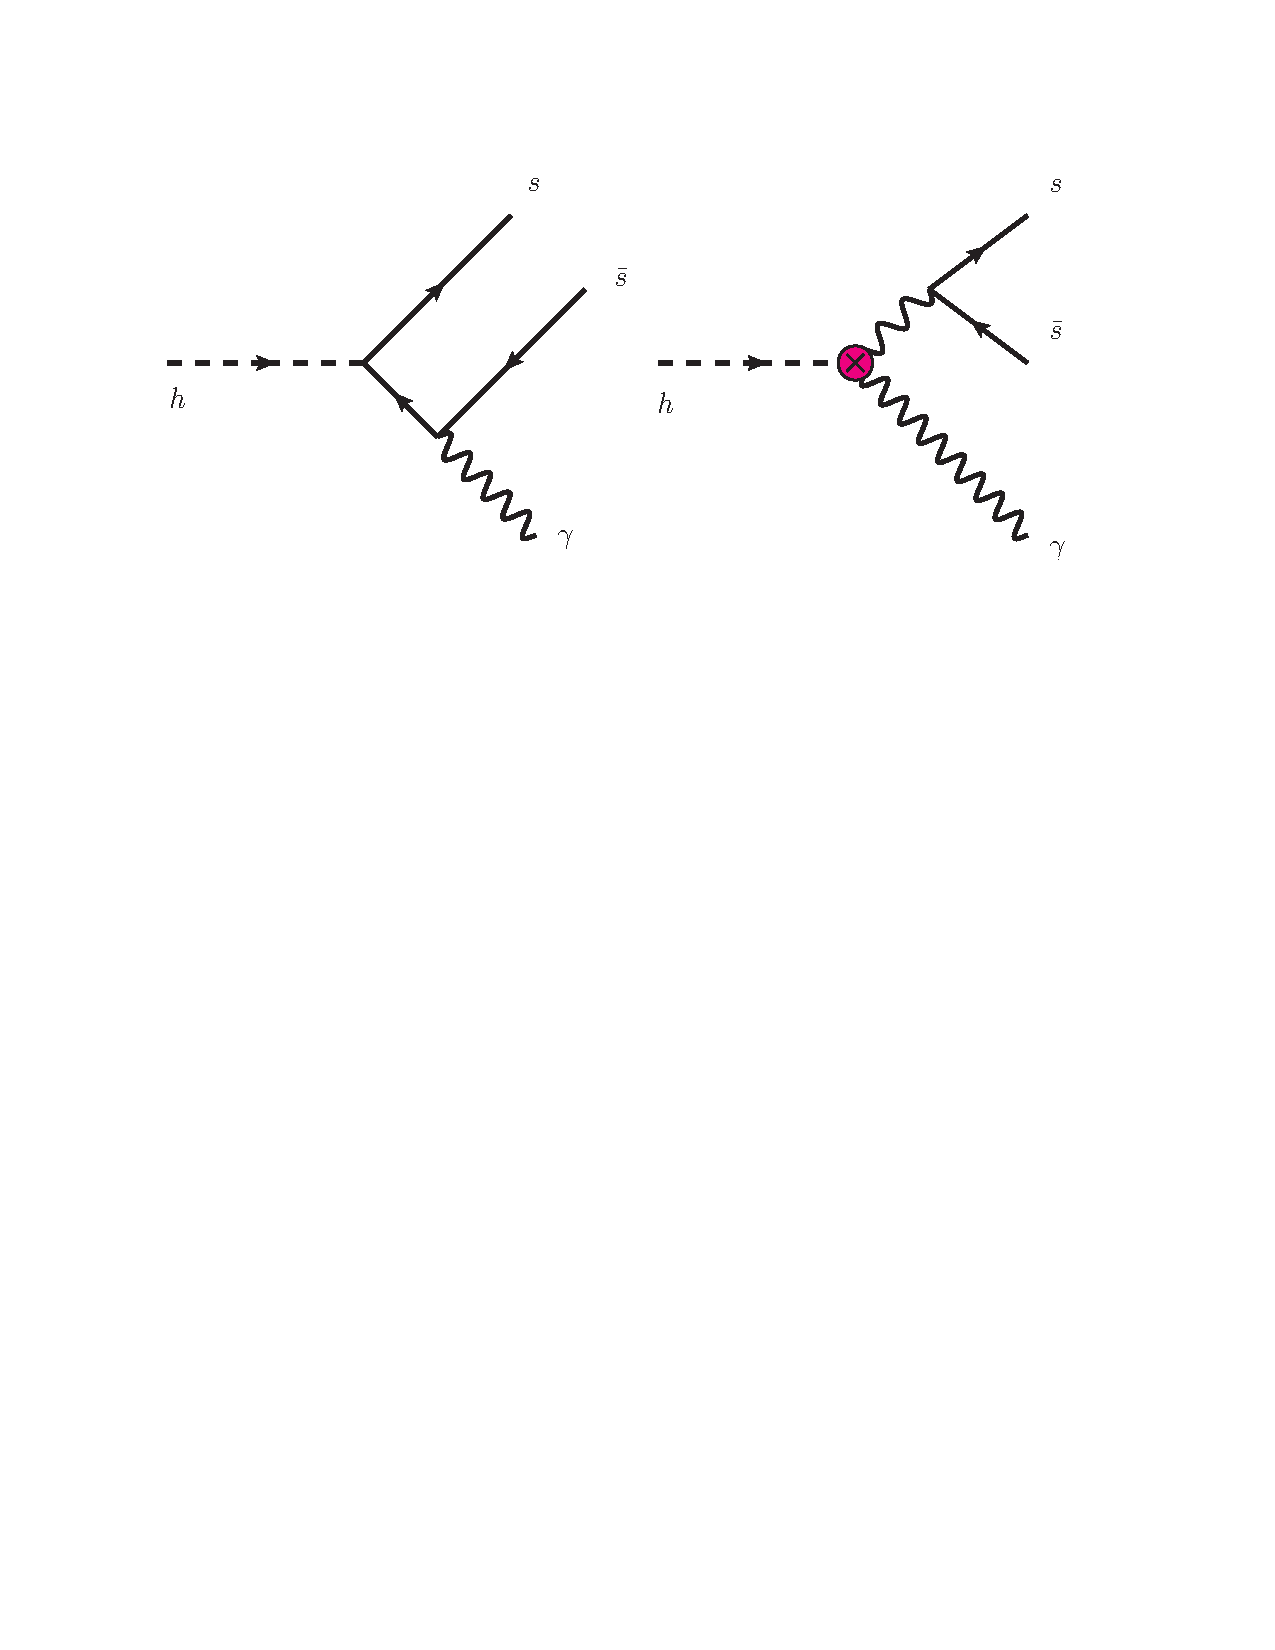
\includegraphics[width=0.65\textwidth]{higgs_exclusive_diag.pdf}
\caption{The two contributions to $h \to V\gamma$ with $V=\rho,\omega,\phi,J/\psi,\Upsilon$. Left: the direct amplitude, proportional to  the $q$-quark Yukawa; Right: indirect amplitude involve the $h\gamma\gamma$ vertex.{\bf YS: replace $s\to q$ the figure}}
\label{fig:hexlusive}
\end{center}
\end{figure}
%%%%%%%%%%%%%%%%%%%%%%%%%%%%%%%%%%%%%%%%%%%%%%%%%%%%%%%%%%%%%%%%%%


It is beneficial to consider the ratio between $h\to V\gamma$ and $h\to\gamma\gamma$ or $h\to ZZ^*\to4\ell$ as various of theoretical uncertainties and the dependence of the Higgs total width are canceled~\cite{Perez:2015aoa,Koenig:2015pha}. Moreover, since the Higgs production is inclusive for all of these modes, it canceled in the ratio to large extension. Thus, we can write 
% 
\begin{align}
	\cR_{V\gamma,f} 
=	\frac{\mu_{V\gamma} }{\mu_{f}}  \frac{ \BR^{\rm SM}_{h\to V\gamma}}{ \BR^{\rm SM}_{h\to f}}  
	\simeq  
	\frac{\Gamma_{h\to V\gamma}}{ \Gamma_{h\to f}}  \, ,
\end{align}
%
where $f=ZZ^*, \gamma\gamma\,$, $\mu_X = \sigma_h \BR_{X}/\sigma^{\rm SM}_h \BR^{\rm SM}_{X}$, the superscript ``SM" denotes the SM values and we assume a perfect cancellation of the production mechanism. 
For simplicity, we assume CP even Higgs coupling and find 
%
\begin{align}
	\cR_{V\gamma,f} 
=& 	\alpha_{V,f} \abs{1 - \left(\Delta^R_V+ i \Delta^I_V \right)\frac{\bar{\kappa}_V}{\kappa^{\rm eff}_{\gamma\gamma}} + \Delta^U_V}^2  \, , 	
\end{align}
%
with
%
\begin{align}	
	\alpha_{V,\gamma\gamma}
=&	6\frac{\Gamma_{V\to e^+e^-}}{\alpha \, m_V} \left( 1 - \frac{m^2_V}{m^2_h} \right)^2 \, , \quad\quad
%
	\alpha_{V,ZZ^*}
= \abs{\frac{\kappa^{\rm eff}_{\gamma\gamma}}{\kappa_{Z}}}^2  \frac{\Gamma^{\rm SM}_{h\to\gamma\gamma}}{\Gamma^{\rm SM}_{h\to ZZ^*\to 4\ell}}\alpha_{V,\gamma\gamma} \, ,
\end{align}
%
where $\kappa_X$ is the normalized coupling with respect to its SM value. Below, we adopted the numerical values of $\Delta^X_V$ from Ref.~\cite{Koenig:2015pha}.
The advantage of use $h\to\gamma\gamma$ for the normalization is that there are only two unknown - the Higgs coupling to di-photon and the quark Yukawa. 
However, since $h\to ZZ^*$ is a very clean channel is serve as a good channel to use for the normalization. 
Moreover, by combing the Higgs data with the electroweak precision measurements, the Higgs coupling to $ZZ$ is known to a few precents level~\cite{Falkowski:2013dza,deBlas:2016ojx}, thus, there is no additional large uncertainty.  
We note that with the current data the bounds evaluating by using $\cR_{V\gamma,ZZ^*}$ are slightly stronger than the ones from $\cR_{V\gamma,\gamma\gamma}$. 

For the interpretation of the experimental results in term of bounds on the different Yukawa coupling we follow Refs.~\cite{Perez:2015aoa,Perez:2015lra}. 
Denoting the 95\,\%\,CL bound on the ratio $\cR_{V\gamma,f}$ as $\cR_{V\gamma,f}^{95}$ we can write 
%
\begin{align}
	\frac{\Delta^R_V - \sqrt{  \frac{(\Delta^R_V)^2 + (\Delta^I_V)^2    }{\alpha_{V\gamma,f}} \cR_{V\gamma,f}^{95}   - (\Delta^I_V)^2 } }{ (\Delta^R_V)^2 + (\Delta^I_V)^2 } 
	< \frac{\bar{\kappa}_V}{\kappa^{\rm eff}_{\gamma\gamma}} < 
	\frac{\Delta^R_V + \sqrt{  \frac{(\Delta^R_V)^2 + (\Delta^I_V)^2    }{\alpha_{V\gamma,f}} \cR_{V\gamma,f}^{95}   - (\Delta^I_V)^2 } }{ (\Delta^R_V)^2 + (\Delta^I_V)^2 }  \, ,
\end{align}
%
where we neglect $\Delta^U_V$ as it is a small correction. 
Moreover, neglecting $\Delta^I_V$ we get simplified formula, which hold to good accuracy, 
%
\begin{align}
	\label{eq:Rsimp}
	\frac{1 - \sqrt{  \cR_{V\gamma,f}^{95}/\alpha_{V\gamma,f} } }{ \Delta^R_V} 
	< \frac{\bar{\kappa}_V}{\kappa^{\rm eff}_{\gamma\gamma}} < 
	\frac{1 + \sqrt{  \cR_{V\gamma,f}^{95}/\alpha_{V\gamma,f} } }{ \Delta^R_V}  \, .
\end{align}
%
Table~\ref{tab:hexclusive} summarizes the current experimental status along with the theory interpretation in terms of light quarks Yukawa.  
%%%%%%%%%%%%%%%%%%%%%%%%%%%%%%%%%%%%%%%%%%%%%%%%%%%%%%%%%%%%%%%%%%
\begin{table}[t]
\begin{center}
\begin{tabular}{|c|c|c|c|}
\hline
mode & $\BR_{h\to V\gamma}<$ & $\cR_{V\gamma,ZZ^*}<$ &Yukawa range  \\
\hline\hline 
$J/\psi\,\gamma$  &
$1.5\times 10^{-3}$\, 8\,TeV~\cite{Aad:2015sda,Khachatryan:2015lga} & 
$9.3$ &
$-295\kappa_Z + 16\kappa^{\rm eff}_{\gamma\gamma} < \kappa_c < 295\kappa_Z + 16\kappa^{\rm eff}_{\gamma\gamma} $\\
\hline
$\phi\,\gamma$ &
$4.8 \times 10^{-4}$\, 13\,TeV~\cite{Aaboud:2016rug,Aaboud:2017xnb} & 
$3.2$ &
$-140\kappa_Z + 10\kappa^{\rm eff}_{\gamma\gamma} < \bar{\kappa}_s < 140\kappa_Z + 10\kappa^{\rm eff}_{\gamma\gamma} $\\
\hline
$\rho\,\gamma$ &
$8.8 \times 10^{-4}$\, 13\,TeV~\cite{Aaboud:2017xnb} & 
$5.8$ &
$-285\kappa_Z + 42\kappa^{\rm eff}_{\gamma\gamma} < 2\bar{\kappa}_u + \bar{\kappa}_d < 285\kappa_Z + 42\kappa^{\rm eff}_{\gamma\gamma} $\\
\hline\hline
\end{tabular}
\end{center}
\caption{The current upper bounds, assuming SM Higgs production, on the different exclusive Higgs decays and the interpretation in terms of the Higgs Yukawa couplings. Note that $\bar{\kappa}_q = y_q/y^{\rm SM}_b\,$. The quoted bounds are at 95\,CL. }
\label{tab:hexclusive}
\end{table}%
%%%%%%%%%%%%%%%%%%%%%%%%%%%%%%%%%%%%%%%%%%%%%%%%%%%%%%%%%%%%%%%%%%


The prospects for probing light quark Yukawa within future LHC runs and for future colliders are estimated in Ref.~\cite{Perez:2015lra}, which we follow here. 
One of the important implications of the first upper bounds on the different exclusive modes is that the measurement is background dominated. Thus, even for future runs, without significant improvement of the analysis, we expect only upper bounds.  
Given an upper bound on $\cR^{95}_{V\gamma,f}(E_1,\cL_1)$, where $E_1\,(\cL_1)$ stands for the collider energy\,(integrated luminosity), the estimated bound with $E_2$ and $\cL_2$ is
%
\begin{align}
	\label{eq:Rscale}
	\cR^{95}_{V\gamma,f}(E_2,\cL_2)
=	\cR^{95}_{V\gamma,f}(E_1,\cL_1) \sqrt{ \frac{1}{R_E} \frac{\sigma^{\rm SM}_{h,E_1} \cL_1  }{\sigma^{\rm SM}_{h,E_2} \cL_2} } \, ,
\end{align}
%
where $\sigma^{\rm SM}_{h,E_{1,2}}$ is the SM Higgs production cross section, $R_{E} = (S_{E_1}^{\rm SM}/B_{E_1})/(S_{E_2}^{\rm SM}/B_{E_2})$ with $S(B)$ the number of signal\,(background) events, which encoded the difference in the analysis details and assumed to be 1 here. 
In Tabel~\ref{tab:exclusiveproj}We combine Eqs.~\eqref{eq:Rsimp} and \eqref{eq:Rscale} along with the current bounds to estimate the future projections of probing the different light quark Yukawa. 
%%%%%%%%%%%%%%%%%%%%%%%%%%%%%%%%%%%%%%%%%%%%%%%%%%%%%%%%%%%%%%%%%%
\begin{table}[t]
\begin{center}
\begin{tabular}{|c|c|c|c|}
\hline
mode & collider energy & $\cR_{V\gamma,ZZ^*}<$ &Yukawa range ($\kappa_V=\kappa^{\rm eff}_{\gamma\gamma}=1$)   \\
\hline\hline 
\multirow{ 3}{*}{$J/\psi\,\gamma$} &
14\,TeV & 
$0.47\sqrt{L_3}$ &
$16 - 67 L_3^{1/4}  < \kappa_c < 16 + 67 L_3^{1/4} $\\
&
27\,TeV & 
$0.28\sqrt{L_3}$ &
$16 - 52 L_3^{1/4}  < \kappa_c < 16 + 52 L_3^{1/4} $\\
&
100\,TeV & 
$0.12\sqrt{L_3}$ &
$16 - 33 L_3^{1/4}  < \kappa_c < 16 + 33 L_3^{1/4} $\\
\hline
\multirow{ 3}{*}{$\phi\,\gamma$} &
14\,TeV & 
$0.33\sqrt{L_3}$ &
$11 - 46 L_3^{1/4} < \bar{\kappa}_s < 11 + 46 L_3^{1/4} $\\
&
27\,TeV & 
$0.20\sqrt{L_3}$ &
$11 - 35 L_3^{1/4} < \bar{\kappa}_s < 11 + 35 L_3^{1/4} $\\
&
100\,TeV & 
$0.083\sqrt{L_3}$ &
$11 - 23 L_3^{1/4} < \bar{\kappa}_s < 11 + 23 L_3^{1/4} $\\
\hline
\multirow{ 3}{*}{$\rho\,\gamma$} &
14\,TeV & 
$0.60\sqrt{L_3}$ &
$44 - 93 L_3^{1/4} < 2\bar{\kappa}_u + \bar{\kappa}_d < 44 + 93 L_3^{1/4} $\\
&
27\,TeV & 
$0.36\sqrt{L_3}$ &
$44 - 72 L_3^{1/4} < 2\bar{\kappa}_u + \bar{\kappa}_d < 44 + 72 L_3^{1/4} $\\
&
100\,TeV & 
$0.15\sqrt{L_3}$ &
$44 - 47 L_3^{1/4} < 2\bar{\kappa}_u + \bar{\kappa}_d < 44 + 47 L_3^{1/4} $\\
\hline\hline
\end{tabular}
\end{center}
\caption{The projection for Yukawa range for future $pp$ colliders with center of mass energy of $14$, $27$ and $100\,$TeV. In the above table we define $L_3\equiv (3/{\rm ab})/\cL\,$. }
\label{tab:exclusiveproj}
\end{table}%
%%%%%%%%%%%%%%%%%%%%%%%%%%%%%%%%%%%%%%%%%%%%%%%%%%%%%%%%%%%%%%%%%%

In addition to the Higgs diagonal Yukawa, in principle, Higgs exclusive decays can probe off-diagonal couplings by measuring modes such as $h\to B^*_s \gamma$~\cite{Kagan:2014ila}. 
These processes receive contribution only from the direct amplitude and there is not enhancement from interference with the relative large indirect amplitude. 
Moreover, the Higgs flavor violating couplings are strongly constrained by meson mixing~\cite{Blankenburg:2012ex,Harnik:2012pb}. Thus, the expected rates are too small to be observe. 
For a detailed discussion on the $h \to VZ,VW$ channels see~\cite{Alte:2016yuw}.



\subsection{Flavor tagging (charm and strange)}

\begin{center}{\emph{$H \rightarrow c \bar{c}$ from charm-tagging, by Emmanuel Stamou}} \end{center}

In the SM, the coupling of the Higgs to bottom quarks is small, i.e.,
$y_b^{\text{SM}}\simeq 0.016$ at $\mu=m_H$, and 
its coupling to charm quarks even smaller by roughly four times,
i.e., $y_c^{\text{SM}}\simeq 0.0036$ at $\mu=m_H$.
Nevertheless, due to phase-space the process $H\to b\bar b$ is the dominant 
decay mode of the Higgs in the SM.
This situation has not only made a roughly $30\%$ precise measurement of such 
a small coupling possible at Run I of the LHC, but has also created 
opportunities to measure possible order one deviations in the 
coupling of the Higgs to charm quarks.

An important difference between the charm- and to some extend also 
the strange-quark (see section \ref{}) with respect to up- and 
down-quarks is that it is possible to pursue an inclusive approach in
identifying the flavour of the final state particles by $c$-tagging jets.
The underlying geometrical/kinematic input necessary for $c$-tagging
is similar to $b$-tagging with the most relevant one being the identification
of displaced vertices due to the lifetime of $c$-hadrons.
$c$-tagging has been used early on in Run I of the LHC by ATLAS in 
searches for supersymmetry, e.g., Refs.~\cite{Aad:2014nra,Aad:2015gna}.
Its usefulness in relations to Higgs physics was first discussed 
in Ref.~\cite{Delaunay:2013pja} and subsequently
used in Ref.~\cite{Perez:2015aoa} to recast ATLAS's and CMS's Run I 
analyses for $h\to b\bar b$ to provide the first LHC 
constraint on the charm Yukawa. 

The inclusive method of probing the charm-quark Yukawa is in many ways complementary 
to searches for exclusive decays (see discussion of section \ref{}) or 
searches for deviations in Higgs distributions (see section \ref{}).
For example, in the inclusive approach an underlying assumption is 
that the Higgs coupling to $WW$ and $ZZ$ ---entering Higgs production--- is SM-like,
while the interpretation of Higgs distributions
assumes no additional new physics contribution that affects them in a significant way.
An important difference between the inclusive and the exclusive approach 
is that the latter relies on interference with the SM $H\to \gamma\gamma$ 
amplitude while the former not.
Therefore, in principle the exclusive approach may be sensitive to the sign and 
$CP$ properties of the coupling to which the inclusive approach is insensitive to.
At the same time, measurements of exclusive decays of the Higgs are challenging due 
to the small probability of fragmenting into the specific final state and 
large QCD backgrounds, which is why the inclusive approach appears to be the most promising
one to probe deviations in the magnitude of the Higgs to charm coupling.

\begin{figure}[h]
	\centering
	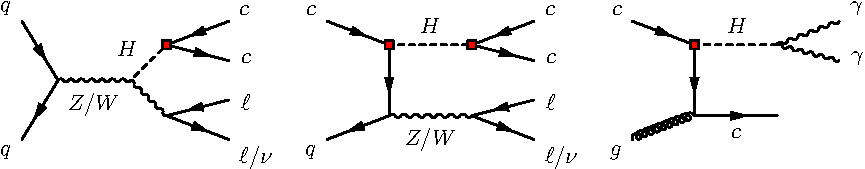
\includegraphics[width=\textwidth]{\main/section7/higgs_production}
	\caption{Left panel, leading-order production of Higgs in association with a heavy gauge boson ($Z/W$) and 
		subsequent decays. Central panel, additional production channel of Higgs in association 
		with a heavy gauge boson that becomes relevant for large $y_c$ \cite{Perez:2015aoa}.
		Right panel, leading-order diagram to search for non-SM $y_c$ in Higgs production in 
		association with a charm-quark \cite{Brivio:2015fxa}.
	\label{fig:higgsproductionHcc}
	}
\end{figure}

The most straight-forward way of inclusively probing the charm-quark Yukawa is by 
expanding the search for $H\to b\bar b$ to search for 
$pp \to (Z/W\to\ell\ell/\nu) (H\to c\bar c)$ \cite{Perez:2015aoa}
(left and central panel in Fig.~\ref{fig:higgsproductionHcc}).
Another possibility discussed in Ref.~\cite{Brivio:2015fxa} is to search for deviations in Higgs production 
in association with a charm quark in which the Higgs is produced from a charm-quark in the proton 
parton-distribution functions (right panel in Fig.~\ref{fig:higgsproductionHcc}).
We focus here on the measurement from $pp\to VH$ events proposed in Ref.~\cite{Perez:2015aoa}
and recently performed on a $36.1$~fb$^{-1}$ sample of $ZH$ data by ATLAS \cite{Aaboud:2018fhh}
at $\sqrt{s}=13$~TeV.
Two key elements for this measurement, which we discuss below, are:
\begin{itemize}
	\item[i)] The experimental sensitivity in discriminating between $c$-jets from
		background $b$- and light-jets.
	\item[ii)] Probing the charm-quark coupling independent of the value of the 
		bottom-quark Yukawa (breaking the degeneracy).
\end{itemize}

\begin{figure}[h]
	\centering
	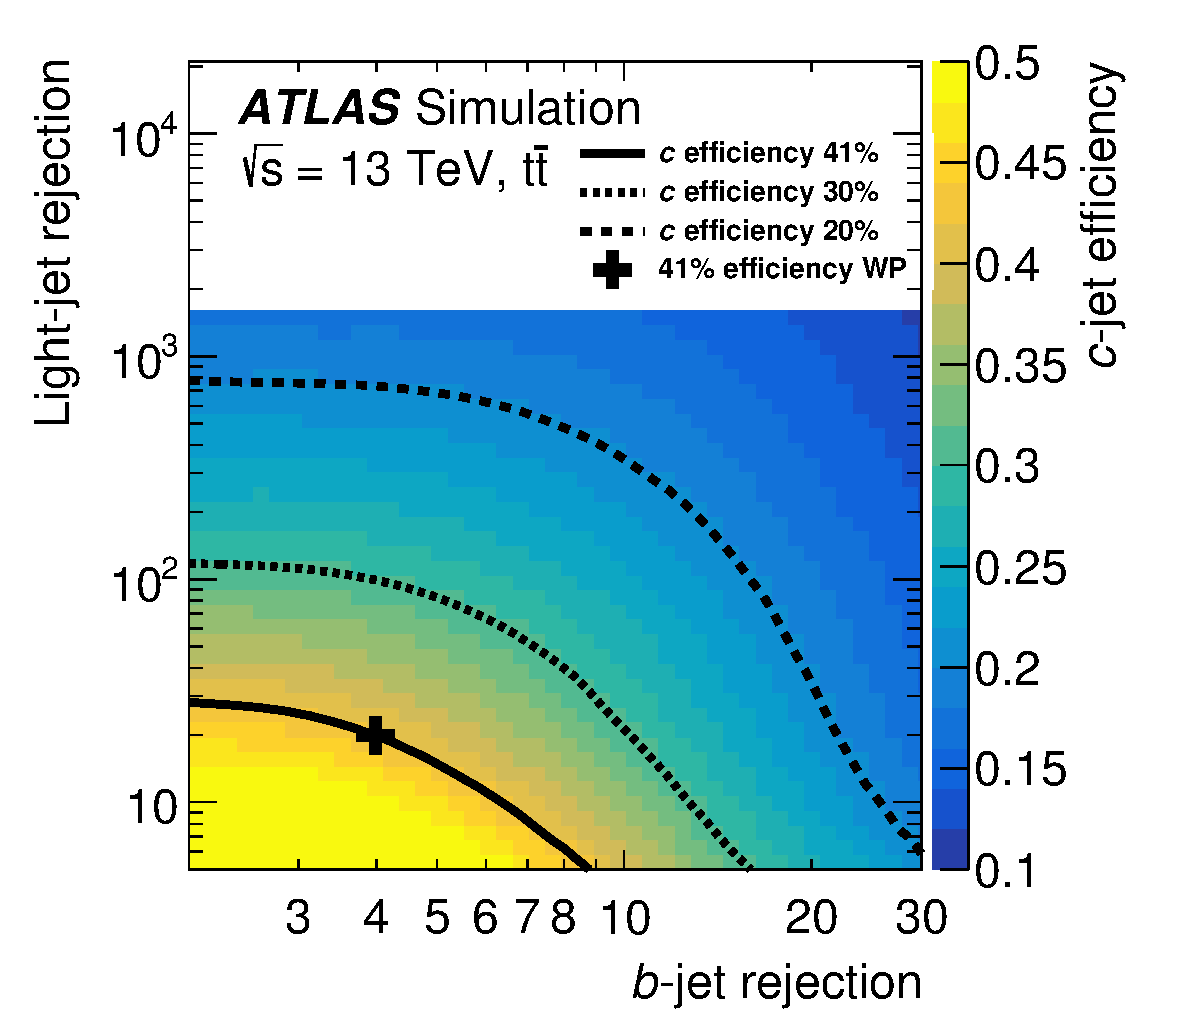
\includegraphics[width=0.4\textwidth]{\main/section7/atlas_efficiency_fig_01}
	\caption{Correlation of $c$-tagging efficiency with $b$- and light-quark-jet rejection
	in ATLAS's $c$-tagger employed in the analysis of Ref.~\cite{Aaboud:2018fhh}.
\label{fig:ATLASctagefficiency}}
\end{figure}

{i)} Tagging algorithms rely on monte-carlo simulations in order to assign a probability 
for a given jet to be produced from a specific quark-flavour. 
Therefore, the efficiency / confidence in associating a jet to a specific quark is 
correlated with the confidence to reject other hypotheses, e.g., production from light-quarks.
ATLAS's recent search \cite{Aaboud:2018fhh} demonstrated that its 
$c$-tagging capabilities are significantly stronger than anticipated.
For LHCb's capabilities of $c$-tagging and its sensitivity to 
$H\to c\bar c$ see section~\ref{}.
The tagging working point chosen in ATLAS's search has an approximately $41\%$ efficiency 
to tag $c$-jets and rejection factors of roughly $4$ and $20$ for $b$- and light-quark-jets, respectively.
In Figure~\ref{fig:ATLASctagefficiency} we show ATLAS's results \cite{Aaboud:2018fhh} 
of the correlation between $c$-tagging efficiency and rejection factors.
This ATLAS result provides to date the most stringent limit in direct searches 
for the inclusive decay of Higgs boson to charm quarks, 
$\sigma(pp\to ZH)\text{BR}(H\to c\bar c)<2.7$\,pb at $95\%$ CL.
To translate this cross-section bound to a non-trivial constraint on $y_c$ it is essential 
to include the additional production channel from large charm Yukawa 
(central panel in Fig.~\ref{fig:higgsproductionHcc}) as demonstrated in Refs.~\cite{Perez:2015aoa}.
The additional production channel is affected by the kinematics, e.g., $p_T$ of the 
$Z$ and thus depends on the details of the analysis. 
This ``unfolding'' / reinterpretation of the analysis is thus best performed by 
the analysis itself and cannot be avoided to obtain non-trivial constraints on the Yukawa itself.
Note that at the moment the systematic uncertainties are approximately a factor of two
larger than the statistical uncertainties of the $36.1$\,fb$^{-1}$ sample used in the analysis;
the largest systematic uncertainty is associated to flavour-tagging and the tagging of $c$-jets 
in particular.

{ii)} Given the rather similar lifetime of $b$ and $c$ hadrons, there is always
a non-negligible ``contamination'' of the $c$-jet sample 
from jets originating from $b$ quarks \cite{Perez:2015aoa}.
An inclusive $H\to c\bar c$ analysis probing $y_c$ must thus either assume a SM value 
for the bottom Yukawa (as assumed in Ref.~\cite{Aaboud:2018fhh}) or allow the 
simultaneous variation of $y_b$ and $y_c$, and break the degeneracy in another way.
As discussed and demonstrated in Refs.~\cite{Perez:2015aoa,Perez:2015lra} this is 
possible by employing more than one tagging working points with a different 
ratio of $c$-tagging efficiency to $b$-jet rejection.
In this way, it possible to gain sensitivity to the two independent contributions 
that enter the search's signal strength, i.e., $\mu_c$ and $\mu_b$.
Though possible this has not been done in ATLAS's latest $13$ TeV search.
It is, however, encouraging that the results presented there would only be mildly 
affected by this (see discussion within Ref.~\cite{Aaboud:2018fhh}).

\begin{figure}[]
	\centering
	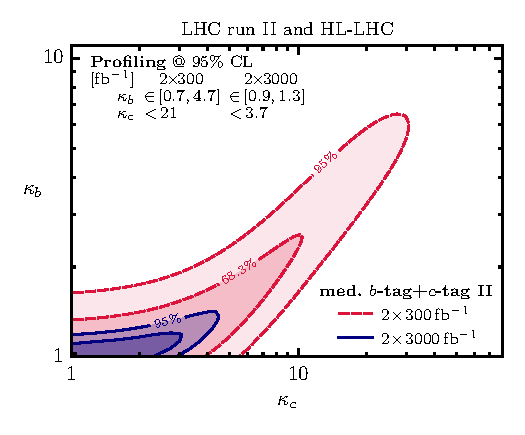
\includegraphics[width=0.45\textwidth]{\main/section7/plot_chi2_14TeV_kappabkappac_A_ctagII}
	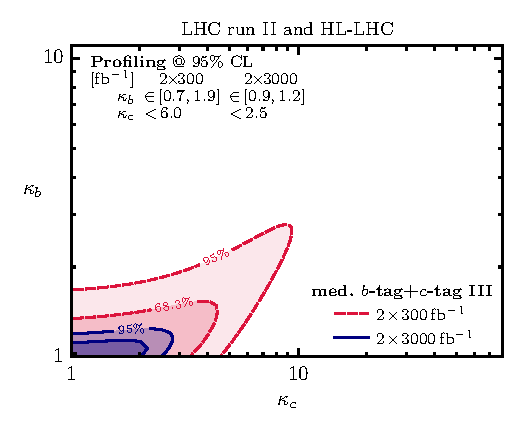
\includegraphics[width=0.45\textwidth]{\main/section7/plot_chi2_14TeV_kappabkappac_A_ctagIII}
	\caption{Projections for measuring charm Yukawa modifications from an inclusive 
		$H\to c\bar c$ search at $\sqrt{s}=14$\,TeV using two different 
		$c$-taggers (left and right panel) \cite{Perez:2015lra}.
		In red the $95\%$ CL region employing an integrated luminosity 
		of $2\times 300$~fb$^{-1}$ and in blue the region 
		employing $2\times 3000$~fb$^{-1}$.
	\label{fig:inclusiveforecast}}
\end{figure}

At the moment there is one official study for the prospects of measuring 
the rate of $pp\to ZH(\to c\bar c)$ from ATLAS \cite{ATL-PHYS-PUB-2018-016}.
The study uses the Run II analysis \cite{Aaboud:2018fhh} to rescale the results 
to the high-luminocity stage of the LHC, i.e., $3000$~fb$^{-1}$, and 
points out directions to imporove on the systematic uncertainties.
The analysis finds that, if there is no significant NP contribution, 
ATLAS will be able to set an $95\%$ CL upper bound on the signal strength 
at a level of $\mu_{ZH(c\bar)} <6.3$.
Yet the collaboration has not unfolded the results to interpret them as 
limits on the charm Yukawa,
for which the additional production mechanism must be included (see above).
To illustrate this point we quote here some results from Ref.~\cite{Perez:2015lra}
in which ATLAS's study of the prospects for measuring $H\to b\bar b$ at $\sqrt{s}=14$\,TeV 
\cite{ATLAS-collaboration:2012iza} has been employed to recast 
the results to an inclusive measurement of $H\to c \bar c$ from Higgs production in 
association with a $Z$ or $W$ boson.
In Figure~\ref{fig:inclusiveforecast} we show the result of the analysis of Ref.~\cite{Perez:2015lra}.
In the left, right panel, a $c$-tagging efficiency of $30\%$ ($c$-tag I), $50\%$ ($c$-tag II) 
was employed, respectively. 
In both cases the $b$-jet rejection was chosen to be $5$ and the light-jet rejection
$200$.
These two tagging working points cover the currently employed tagging working point in which
the $c$-tagging efficiency is approximately $41\%$.
In the analysis both the charm and the bottom quark are treated as free variables;
the bottom-Yukawa direction is profiled away to project the sensitivity to the 
charm-quark Yukawa.
It was found that with $2\times 3000$\,fb$^{-1}$ at $\sqrt{s}=14$\,TeV the 
high-luminocity stage of the LHC probes values of $y_c/y_c^{\text{SM}}\simeq 21,\,6$ with
$c$-tag I (left panel), $c$-tag II (right panel) at $95\%$ CL 
(the blue regions in Figure~\ref{fig:inclusiveforecast}).
The recent ATLAS analysis has studied the systematic uncertainties associated 
to such measurements, in particular the uncertainties associated to $c$-tagging.
Such uncertainties could not have been included in the above initial analysis of
the future study, but are to a large extend include in ATLAS's study \cite{ATL-PHYS-PUB-2018-016}.


\begin{center}{\emph{$H \rightarrow c \bar{c}$ at LHCb, by Oscar Augusto De Aguiar Francisco and Lorenzo Sestini}} \end{center}

Even though the LHCb experiments operates at lower luminosity when compared to ATLAS/CMS, it has unique capabilities for discrimination between b- and c-jets thanks to its excellent vertex reconstruction system \cite{Aaij:2015yqa}. Its acceptance covers $\sim 5$\% of the associated production of $W/Z+H$ at 13 TeV. The Figure~\ref{fig:hbbetas} shows the coverage of the LHCb for the $b\bar{b}$ produced by the Higgs decay in association with a vector boson. When the two jets are in acceptance, the lepton from $W/Z$ tends to be in acceptance as well ($\sim 60$\% of times). Due to its forward geometry, more boosted Higgs are more likely to be properly reconstructed.

During the Run I LHCb set experimental upper limits on the $V+H(\rightarrow b \bar{b})$ and $V+H(\rightarrow c \bar{c})$ production \cite{LHCb:2016yxg}.
Neglecting any improvements in the analysis or detector, the extrapolation of the limit obtained at 8 TeV to 300fb$^{-1}$ at 14 TeV is $\sim 50\times$BR(SM) for H($c\bar{c}$). 

Detector improvements are expected in future upgrades, in particular in impact parameter resolution which directly affects the c-tagging efficiency. 
If the detector improvement is taken into account, the c-jet tagging efficiency is expected to be improved as can be seen in the Figure~\ref{fig:c-tag-eff}.  
A further improvement is expected from the electron reconstruction that will benefit from upgraded versions of the electromagnetic calorimeter. Electrons are used in the identification of the vector bosons associated with the Higgs.
Therefore, with these improvements, the expected limit can be pushed down to $5-10\times$BR(SM).
In terms of Yukawa coupling this correspond to limit of 2-3 times the Standard Model prediction.
These extrapolation does not include improvements on analysis techniques: as example a Deep Learning analysis can be applied to exploit the jets substructures properties to reduce the backgrounds.

\begin{figure}[ht]
	\centering
	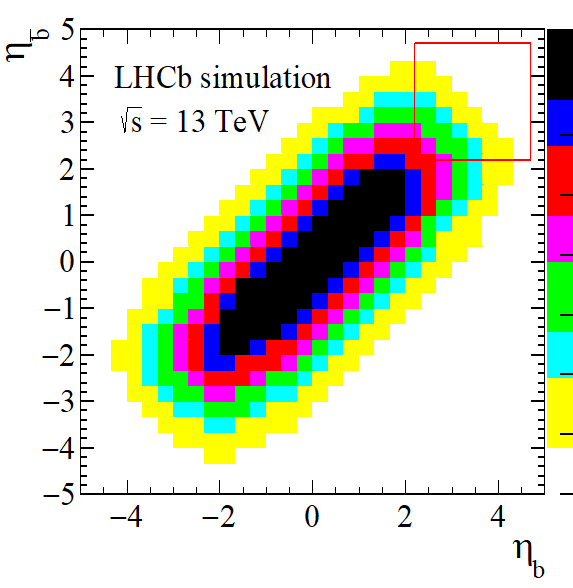
\includegraphics[width=0.5\linewidth]{\main/section7/hbb_etas.png}
	\caption{2D histogram showing the coverage of the LHCb acceptance for the $b\bar{b}$ pair produced by the Higgs decay in associated production with a W or a Z boson.}
	\label{fig:hbbetas}
\end{figure}

\begin{figure}[ht]
	\centering
	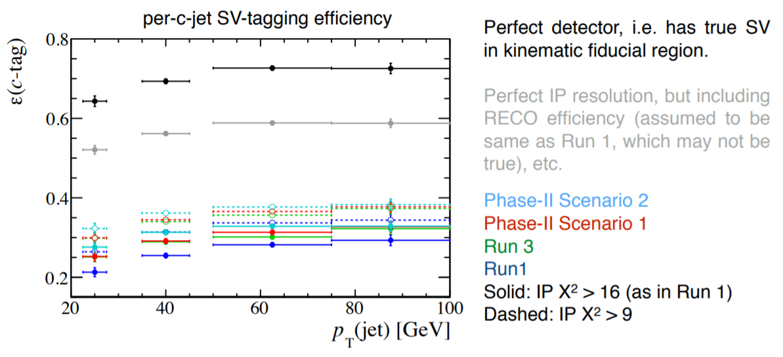
\includegraphics[width=0.99\linewidth]{\main/section7/c-tag-eff.png}
	\caption{c-jet tagging efficiency for different scenarios in the HL-LHC conditions.}
	\label{fig:c-tag-eff}
\end{figure}

\FloatBarrier

\subsubsection{Strange quark tagging}
\label{sec:strange-tagging}

Tagging strange jets from Higgs decays provides an alternative method to exclusive Higgs
decays~\cite{Kagan:2014ila, Perez:2015lra, Koenig:2015pha, Aaboud:2016rug, Aaboud:2017xnb,
  Alte:2016yuw} for constraining the Yukawa coupling of the strange quark. See \Bref{Soreq:2016rae,
  Yu:2016rvv, Bishara:2016jga, Gao:2016jcm} for approaches using event shape and kinematic
observables. The main idea behind the strange tagger described in \Bref{Duarte:2018xyz} is that
strange quarks---more than other partons---hadronize to prompt kaons that carry a large fraction of
the jet momentum. Based on this idea a tagger is constructed to allow for an estimate of the
capabilities in measurements involving strange quarks. Although the current focus at LHC is on
mainly on charm and bottom tagging, recognizing strange jets has been attempted before at
DELPHI~\cite{Boudinov:1998fao} and SLD~\cite{Kalelkar:2000ig}, albeit in $Z$ decays.

The shown results are based on an analysis of event samples of Higgs and $W$ events generated with
\texttt{PYTHIA} 8.219~\cite{Sjostrand:2006za, Sjostrand:2014zea}. In each of the two hemispheres of
the resonance decay, the charged pions and kaons stemming from the resonance are selected with an
assumed efficiency of 95\%. Similarly, $K_s$ are identified with an efficiency of 85\% if they decay
within \Unit{80}{cm} of the interaction point into a $\pi^+\pi^-$ pair that allows to reconstruct
the decaying neutral kaon. Among the two lists of kaon candidates---one per hemisphere---one kaon of
each list is chosen for further analysis such that the scalar sum of their momenta is maximized
while rejecting charged same-sign pairs. The events are separated into the categories
charged-charged (CC), charged-neutral (CN) and neutral-neutral (NN) with a relative abundance of
about CC:CN:NN$\approx 9:6:1$ from isospin considerations and branching ratios by the charges of the
selected kaon candidates.

All selected candidates are required to carry a large momentum $p_{||}$ along the hemisphere
axis. This cut allows to reduce the background from gluon jets as gluons radiate more than quarks
and therefore tend to spread their energy among more final state particles. In addition, charged
kaons need to be produced promptly, in order to reject heavy flavor jets. This latter requirement is
implemented by a cut on the impact parameter $d_0$ after the truth value has been smeared by the
detector resolution.
\begin{figure}[tb]
  \centering
  
\includegraphics[width=0.6\textwidth]{\main/section7/fs_legend}\\
  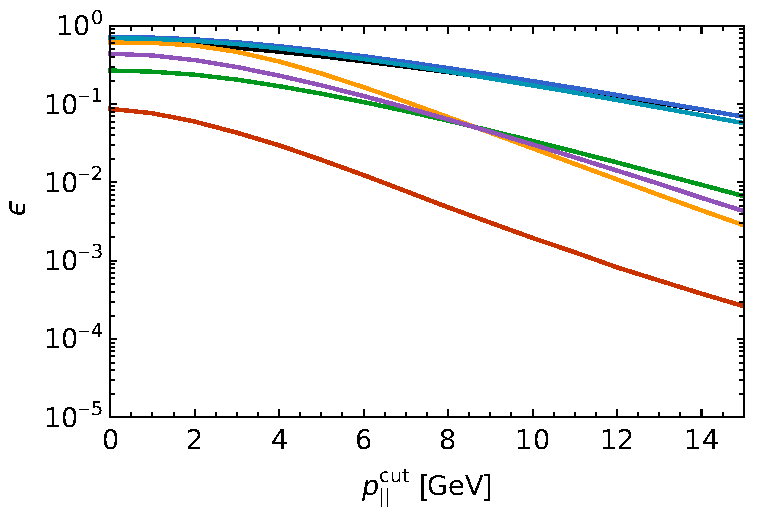
\includegraphics[width=0.49\textwidth]{\main/section7/eff_CC_2s_1_014}
  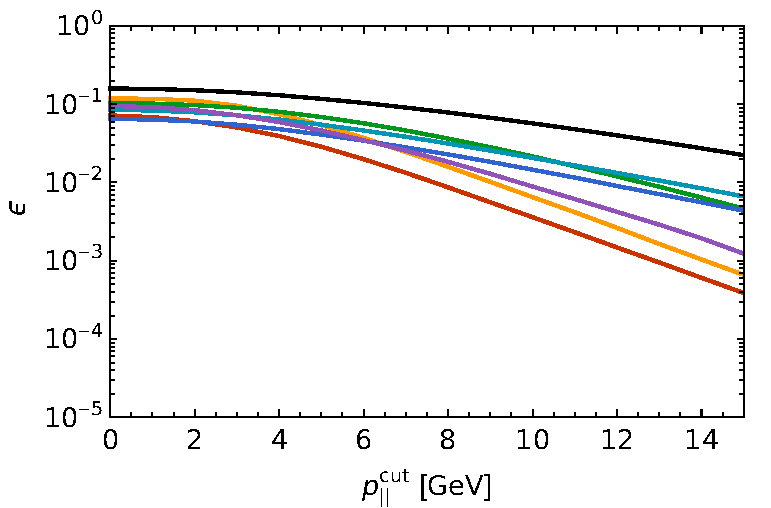
\includegraphics[width=0.49\textwidth]{\main/section7/eff_NC_2s_1_014}
  \caption{Efficiencies as function of the cut on $p_{||}$ and for $d_0<$\Unit{14}{$\mu$m} to
    reconstruct the different Higgs decay channels and $W$ decays as $s\bar s$ event by the
    described tagger. The left plot shows the CC channel, the right the CN channel.}
  \label{fig:stagger-efficiencies}
\end{figure}

The efficiencies obtained in the CC and CN channel for a cut of $d_0<$\Unit{14}{$\mu$m} are shown in
Fig.~\ref{fig:stagger-efficiencies}. While there is clearly still ample room for improvement, this
simple tagger shows already a good suppression by orders of magnitude of the bottom, charm and gluon
background. Due to missing particle identification, the efficiencies for first-generation jets and
strange jets are degenerate in the CC channel. However, in the CN channel, due to the required
$K_s$, a suppression of pions is achieved that breaks this degeneracy. This is particularly
interesting in light of the HL-LHC, where a large background from first generation jets is expected.

\subsection{LFV decays of the Higgs}


\subsection{Yukawa constraints from Higgs distributions}

The Higgs transverse momentum, $p_T$, distributions have been considered before as a probe of high scale new physics running in the $ggh$ loop, see~\cite{Arnesen:2008fb,Biekotter:2016ecg,Brehmer:2015rna,Dawson:2015gka,Schlaffer:2014osa,Grojean:2013nya,Langenegger:2015lra,Bramante:2014hua,Buschmann:2014twa,Azatov:2013xha,Banfi:2013yoa,Buschmann:2014sia}. 
In addition, the soft spectrum is an indirect probe of the Higgs coupling to light quarks~\cite{Soreq:2016rae,Bishara:2016jga}. 
Quark fusion production of Higgs, which is negligible in the SM, have two effects of the Higgs kinematical distributions. 
%
First, the Sudakov peak will be at smaller $p_T$ around 5\,GeV vs 10\,GeV for gluon fusion, see~\cite{Collins:1984kg}. This is because the effective radiation strength of gluon is few times larger than of quarks, $\alpha_s N_c$ vs. $\alpha_s (N^2_c-1)/(2N_c)$, with $N_c=3$. This leads to harder $p_T$ spectrum for gluon fusion than in the quark case. 
In terms of normalized $p_T$ distribution, therefore, the $u\bar{u}$ or $d\bar{d}$ scattering leads to a much sharper peak at lower $p_T$ compared with the $gg$ scattering~\cite{Soreq:2016rae}.
Second, in the SM, the Higgs production is dominated by a gluon fusion, where the two gluon carry similar partonic $x$. This leads to peak at zero Higgs rapidity. However, for $u\bar u$ or $d\bar d$ fusion, the valance quark will carry larger partonic $x$ than the sea anti-quark. This leads to a peak in the forward direction. 
%
For enhanced $s$ or $c$ Yukawa, the dominant effect is the one loop of the quarks in the $gg\to hj$ process, which show double logarithms behavior and peaks toward low Higgs $p_T$~\cite{Baur:1989cm}. This will also resulting in a softer Higgs $p_T$ spectrum~\cite{Bishara:2016jga}, which can be used to constrain the charm and strange Yukawa. 
%
For illustration of the above effect on the different kinematical distributions see In Fig.~\ref{fig:HiggsDist}. 
We comment that many theoretical and experimental uncertainties are canceled in  the normalized kinematical distribution, $(1/\sigma)d\sigma/dX$ with $X=p_T, y_h$, see for example~\cite{Soreq:2016rae}.
Thus, the use of them will result in a better sensitivity for probing the light quark Yukawa. 
%%%%%%%%%%%%%%%%%%%%%%%%%%%%%%%%%%%%%%%%%%%%%%%%%%%%%%%%%%%%%%%%%%
\begin{figure}[t]
\begin{center}
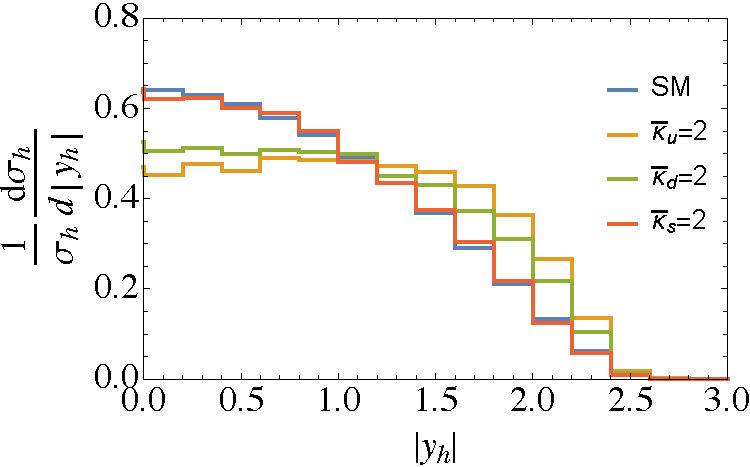
\includegraphics[width=0.35\textwidth]{Disteta.pdf}~~~~~~~~
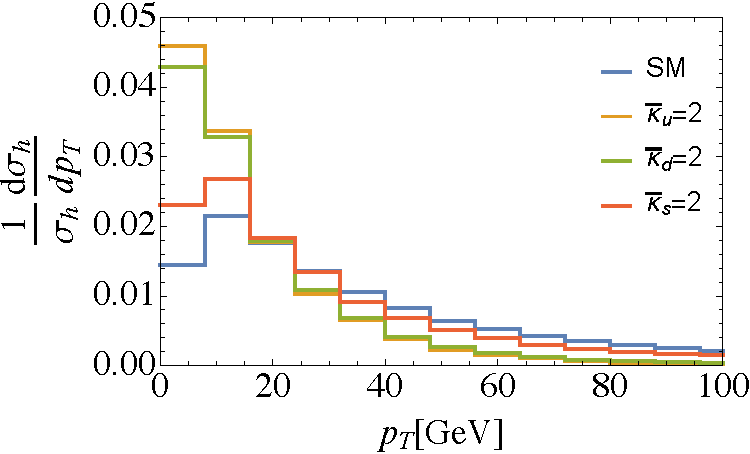
\includegraphics[width=0.35\textwidth]{DistpT.pdf}\\
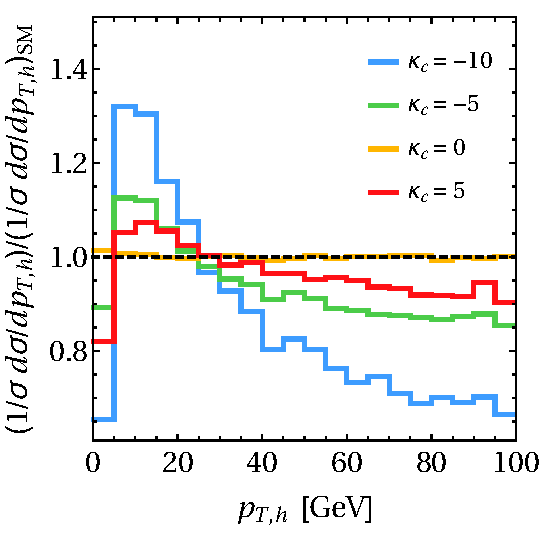
\includegraphics[width=0.35\textwidth]{normalizedcharm8TeV.pdf}
\caption{The Higgs normalized distributions. 
Left-top\,(Right-top) : $y_h\,(p_T)$ distribution for enhanced $u$, $d$ and $s$ Yukawa compared to the SM~\cite{Soreq:2016rae};
Bottom: $p_T$ distribution for enhanced $c$ Yukawa~\cite{Bishara:2016jga}. 
}
\label{fig:HiggsDist}
\end{center}
\end{figure}
%%%%%%%%%%%%%%%%%%%%%%%%%%%%%%%%%%%%%%%%%%%%%%%%%%%%%%%%%%%%%%%%%%

In Ref.~\cite{Soreq:2016rae}, the 8\,TeV ATLAS data~\cite{Aad:2015lha} has been used to evaluate first bound on the $u$ and $d$ Yukawa from the Higgs kinematical distribution. The resulting $95\,\%$ CL regions from the  $p_T$ distribution are
%
\begin{align}
	\bar{\kappa}_u = y_u/y^{\rm SM}_b < 0.46 \, , \qquad\qquad
	\bar{\kappa}_d = y_d/y^{\rm SM}_b< 0.54 \, ,
\end{align}
%
which are stronger than the fits to the inclusive Higgs production cross sections. 
Note that the above upper bound found to be stronger than the expected due to lower fluctuation of the data in the first $p_T$ bin. 
The bounds from the 8\,TeV Higgs rapidity distribution are found to be weaker. 
The sensitivity of the 13\,TeV run of the rapidity and transverse momentum distribution is plotted in Fig.~\ref{fig:HiggsDistFuture}. 
%% add cite to \ys{future projection; cite the latest Higgs $p_T$~\cite{Chen:2018pzu}
%%%%%%%%%%%%%%%%%%%%%%%%%%%%%%%%%%%%%%%%%%%%%%%%%%%%%%%%%%%%%%%%%%
\begin{figure}[t]
\begin{center}
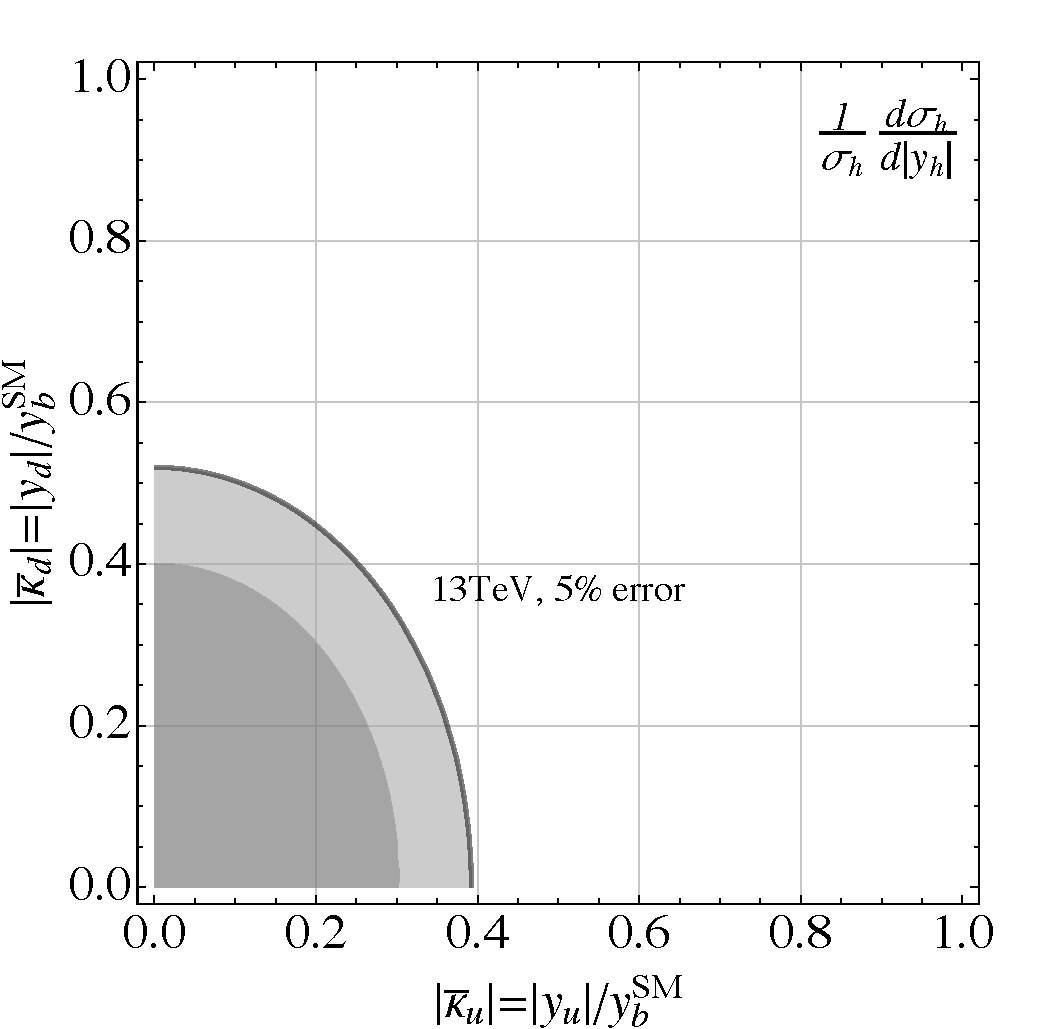
\includegraphics[width=0.35\textwidth]{Naive13TeVy.pdf}~~~~~~
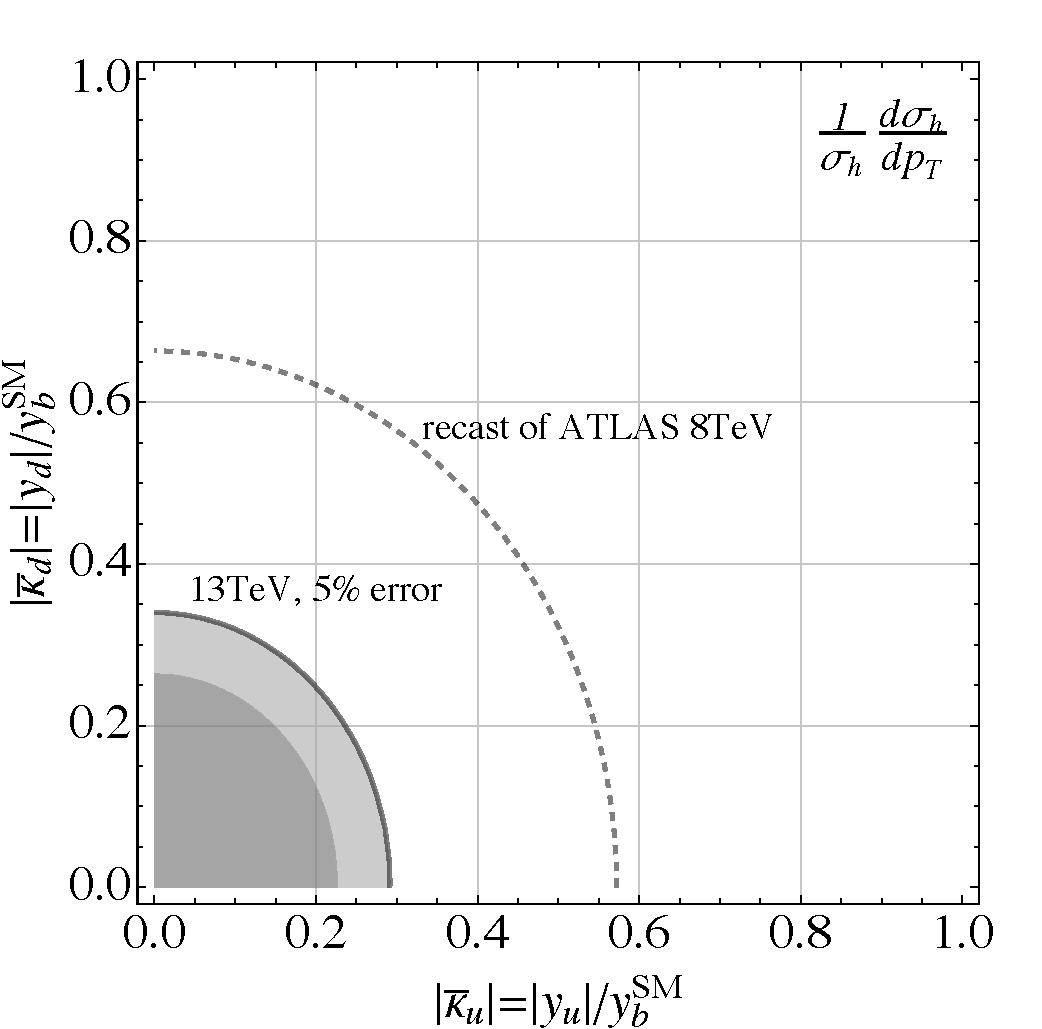
\includegraphics[width=0.35\textwidth]{Naive13TeVpT.pdf}\\
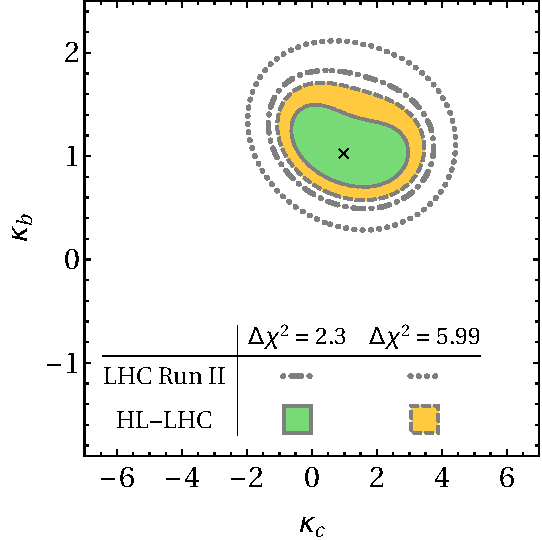
\includegraphics[width=0.35\textwidth]{future12.pdf}
\caption{The sensetivy of the different angular distribution to probe light quarks Yukawa at 13\,TeV.  
Left-top: $u$ and $d$ quark Yukawa from $y_h$ distribution~\cite{Soreq:2016rae};
Right-top: $u$ and $d$ quark Yukawa from $p_T$ distribution~\cite{Soreq:2016rae}; 
Bottom: $b$ and $c$ quark Yukawa from $p_T$ distribution~\cite{Bishara:2016jga}. 
}
\label{fig:HiggsDistFuture}
\end{center}
\end{figure}
%%%%%%%%%%%%%%%%%%%%%%%%%%%%%%%%%%%%%%%%%%%%%%%%%%%%%%%%%%%%%%%%%%

Following Ref.~\cite{Bishara:2016jga}, CMS interpertated the 13\,TeV Higgs $p_T$ spectrum with luminoisty of $35.9\,$fb$^{-1}$ as bounds on the $c$ and $b$ Yukawa~\cite{CMS:2018hhg}. In case that the branching ratio are allowed to floated\,(are depend on $\kappa_c$ and $\kappa_b$), the resulting 95\,\% CL intervals are
%
\begin{align}
    -2.8\,(-0.9) < \kappa_c < 9.9\,(0.9) \, , \qquad
    -18.0\,(-4.3) < \kappa_b < 22.9\,(4.3) \, .
\end{align}
%
These bounds on the $c$ Yukawa are weaker\,(stronger) then the bounds from the global fit of the 8\,TeV Higgs data along with the electroweak precision data allowing all Higgs coupling to float~\cite{Perez:2015aoa}  

\subsubsection{Determinations of Higgs boson coupling modifiers using differential distributions}

{\it this subsection contributed by T. Klijnsma (integrated by A.Schmidt) on 5. Oct. for CMS. It still needs to be merged with the section above}


Variations of Higgs boson couplings alter the SM Higgs production cross sections, both inclusively and differentially.
% 
Exploiting the deviations of the differential spectra, in particular the transverse momentum spectrum, $\pth$, one can constrain Higgs boson couplings using information that is not available in inclusive measurements~\cite{%
Khachatryan:2016vau,% 7 & 8 TeV coupling combination
Aad:2015zhl,% 7 & 8 TeV mass combination
CMS:2018lkl% 13 TeV CMS coupling combination
}.
% 
As the measurements of differential cross sections are generally dominated by statistical uncertainties~\cite{CMS-PAS-HIG-17-028}, these constraints are expected to improve drastically with the advent of more data.



The Higgs boson couplings are free parameters in the SM Lagrangian, and there are many potential extensions of the SM~\cite{Dimopoulos:1981zb,Witten:1981nf} that predict deviations of their SM values.
% 
Using the transverse momentum distribution measured by the ATLAS Collaboration at $\sqrt{s}=8$\TeV~\cite{Aad:2015lha}, corresponding to an integrated luminosity of $20.3$\fbinv, for the first time limits were set on the coupling to the charm quark, $\kappac$, using differential distributions~\cite{Bishara:2016jga}.
% 
These limits are compatible with those obtained from direct limits, such as a search using the same dataset for $\PH\to\jpsi\photon$ by the ATLAS Collaboration~\cite{Aad:2015sda}, and a search for $\hcc$ by the ATLAS Collaboration~\cite{Aaboud:2018fhh} using data collected at $\sqrt{s}=13$\TeV, corresponding to an integrated luminosity of $36.1$\fbinv.
% 
In addition to this study of the Higgs boson coupling to light quarks concerning mostly $\pth \lessapprox \mH$ (where $\mH$ is the Higgs boson mass), a study~\cite{Grazzini:2017szg,Grazzini:2016paz} involving simultaneous variations of the Higgs boson coupling to the top quark, $\kappat$, the bottom quark, $\kappab$, and an anomalous direct coupling to the gluon field, $\cg$, aims to exploit the tails of the $\pth$ distribution.



Differential Higgs boson production cross section measurements are available from both the ATLAS~\cite{%
Aad:2014lwa,% diff. ATLAS hgg, Run I
Aad:2014tca,% diff. ATLAS hzz, Run I
Aad:2016lvc,% diff. ATLAS hww, Run I
Aaboud:2018xdt,% diff. ATLAS hgg, Run II
Aaboud:2017oem,% diff. ATLAS hzz, Run II
Aaboud:2018ezd% diff. ATLAS combination Run II    
} and CMS~\cite{%
Khachatryan:2015rxa,% diff. CMS hgg, Run I
Khachatryan:2015yvw,% diff. CMS hzz, Run I
Khachatryan:2016vnn,% diff. CMS hww, Run I
Sirunyan:2018kta,% diff. CMS hgg, Run II
CMS_AN_2016-442,% diff. CMS hzz, Run II
CMS-PAS-HIG-17-028% diff. CMS combination Run II
} Collaborations at $\sqrt{s}=8$ and $13$\TeV.
% 
Recently, the \hyphenation{parametrized} theoretical predictions of the $\pth$ distribution from Ref.~\cite{Bishara:2016jga} and Refs.~\cite{Grazzini:2017szg,Grazzini:2016paz} were fitted to data~\cite{CMS-PAS-HIG-17-028} collected by the CMS Collaboration at $\sqrt{s}=13$\TeV, corresponding to an integrated luminosity of $36.1$\fbinv.
% 
This section concerns the projection of the constraints on Higgs boson couplings obtained in Ref.~\cite{CMS-PAS-HIG-17-028} to an integrated luminosity of $3000$\fbinv.
% 
We report projections for the simultaneous fits to data of $\kappac$ and $\kappab$ and of $\kappat$ and $\cg$, using projections of the differential distributions at $3000$\fbinv obtained elsewhere \textbf{[Ref to pure diff xs projection here]}.



The Higgs boson coupling fits are based a combination of $\pth$ distributions from the $\hgg$~\cite{Sirunyan:2018kta} and $\hzztofourl$~\cite{CMS_AN_2016-442} (where $\ell = \electron$ or $\muon$) decay channels obtained at $\sqrt{s}=13\,$TeV.
% 
Furthermore, a search for the Higgs boson produced with large \pt and decaying to a bottom quark-antiquark ($\bb$) pair~\cite{CMS_AN_2016-366}, which enhances the sensitivity at high $\pth$, is included in the $\kappat/\cg$ fit.
% 
The Higgs boson coupling fits are performed using an simultaneous extended maximum likelihood fit to the diphoton mass, four-lepton mass, and soft-drop mass $\msd$~\cite{Dasgupta:2013ihk,Larkoski:2014wba} spectra in all the analysis categories of the $\hgg$, $\hzz$, and $\hbb$ channels, respectively.
% 
For more details on the treatment of the input measurements, see Ref.~\cite{CMS-PAS-HIG-17-028}.



The treatment of the decay of the Higgs boson affects the Higgs boson coupling fits.
% 
Assuming full knowledge of how the Higgs decays, \ie assuming no beyond-the-SM contributions, the inclusive Higgs production cross section adds a strong constraint on the Higgs boson couplings in the fit.
% 
This result is obtained by parametrizing the branching fractions as functions of the Higgs boson couplings.
% 
Likewise, the constraints on the Higgs boson couplings excluding the information from the inclusive cross section are of interest in order to evaluate the discriminating power of the differential distributions.
% 
This result is implemented by letting the branching fractions be determined in the fit without any prior constraint.



The expected one and two standard deviation contours of the $\kappac/\kappab$ fit with the branching fractions \hyphenation{parametrized} as functions of the Higgs boson couplings at a projected integrated luminosity of $3000$\fbinv is shown in Fig.~\ref{fig:kbkc_couplingdependentBRs}, for both scenarios of systematic uncertainty.
% 
For the $\hgg$ channel the systematic uncertainties dominate if kept at the current level (\ie in Scenario 1), but when scaled down according to the Scenario 2 prescription the systematic uncertainties are within the same order of magnitude as the statistical ones.



The same fits, but now with the branching fractions implemented as nuisance parameters with no prior constraint, are shown in \ref{fig:kbkc_floatingBRs}.
% 
As this fit is dominated by statistical uncertainties even at very high integrated luminosities, the smaller systematic uncertainties in Scenario 2 have only a minor impact.



\begin{figure}[hbtp]
  \begin{center}
    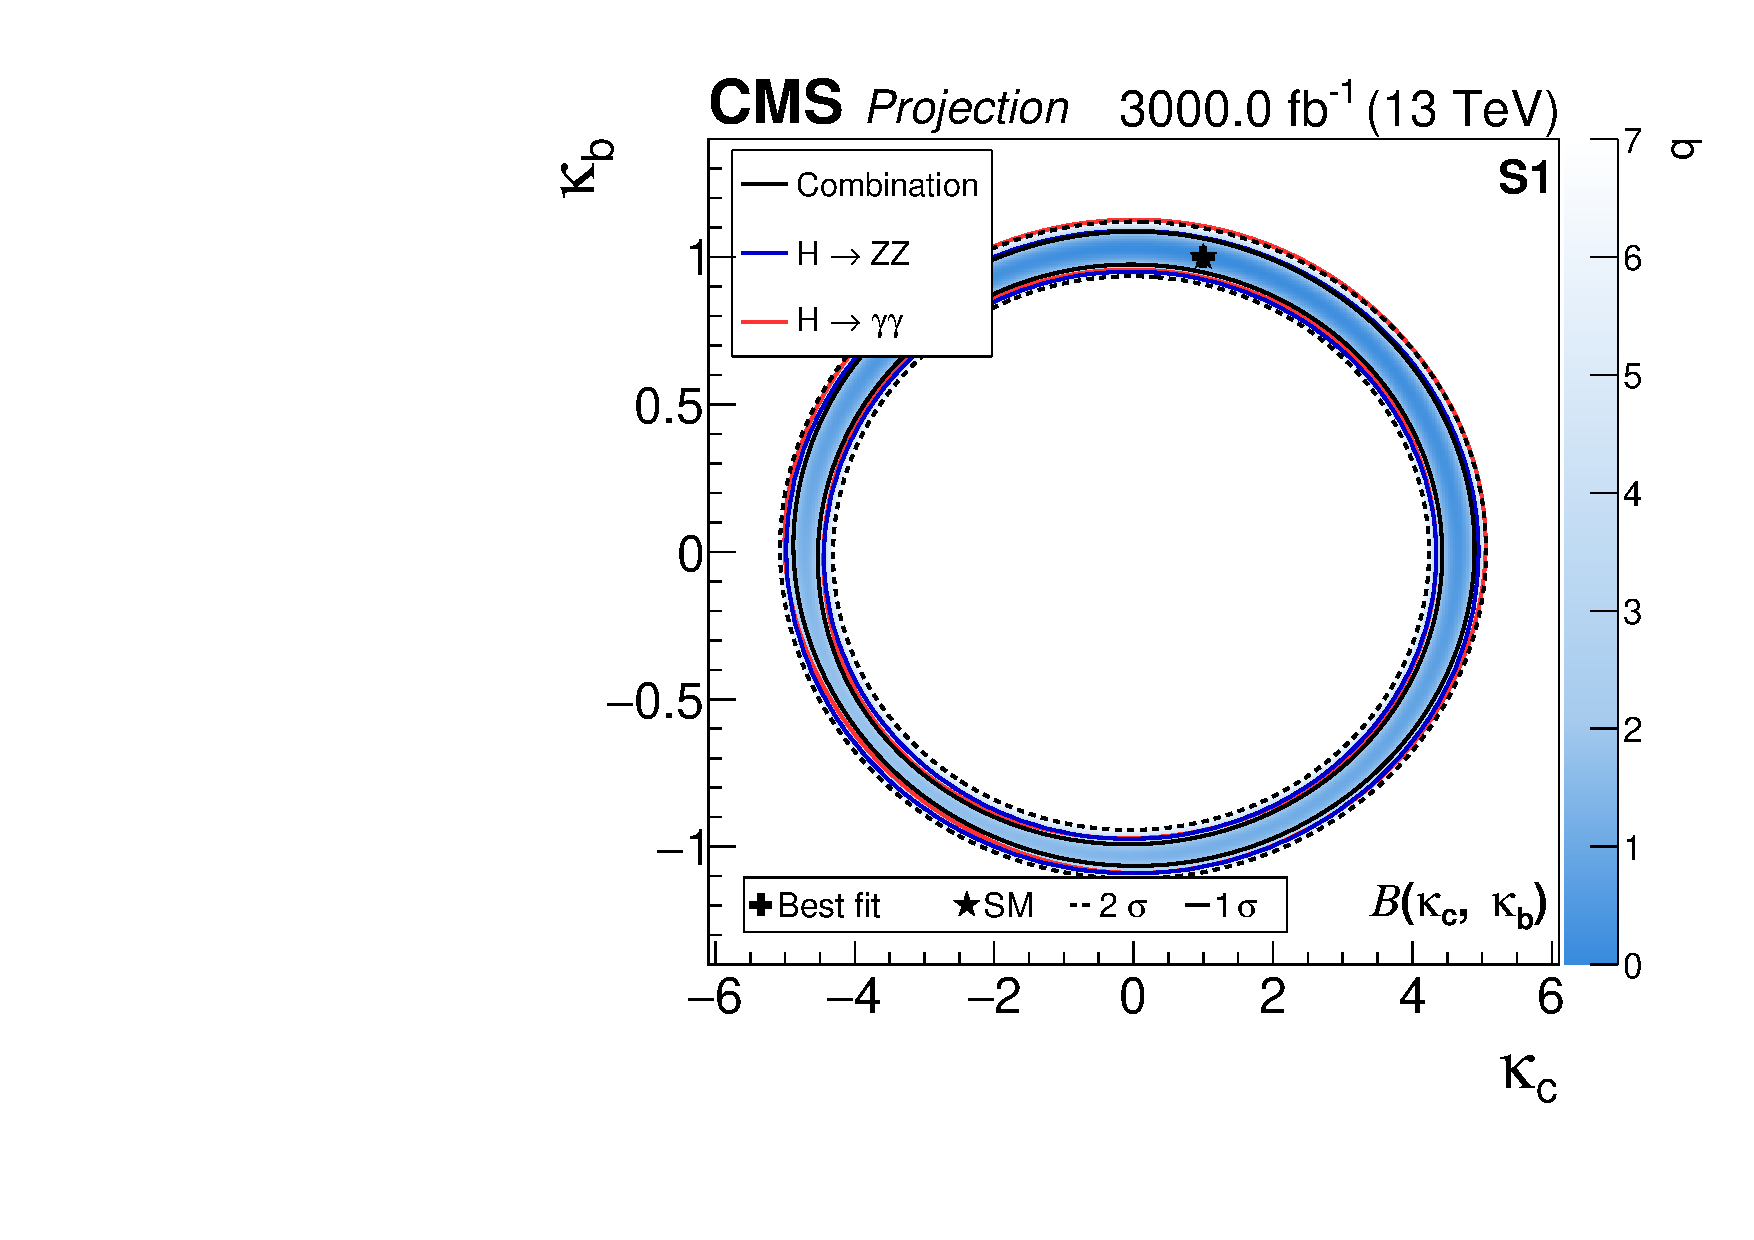
\includegraphics[width=0.49\linewidth]{\main/section7/projection_kbkc_plot_couplingdependentBRs.pdf}
    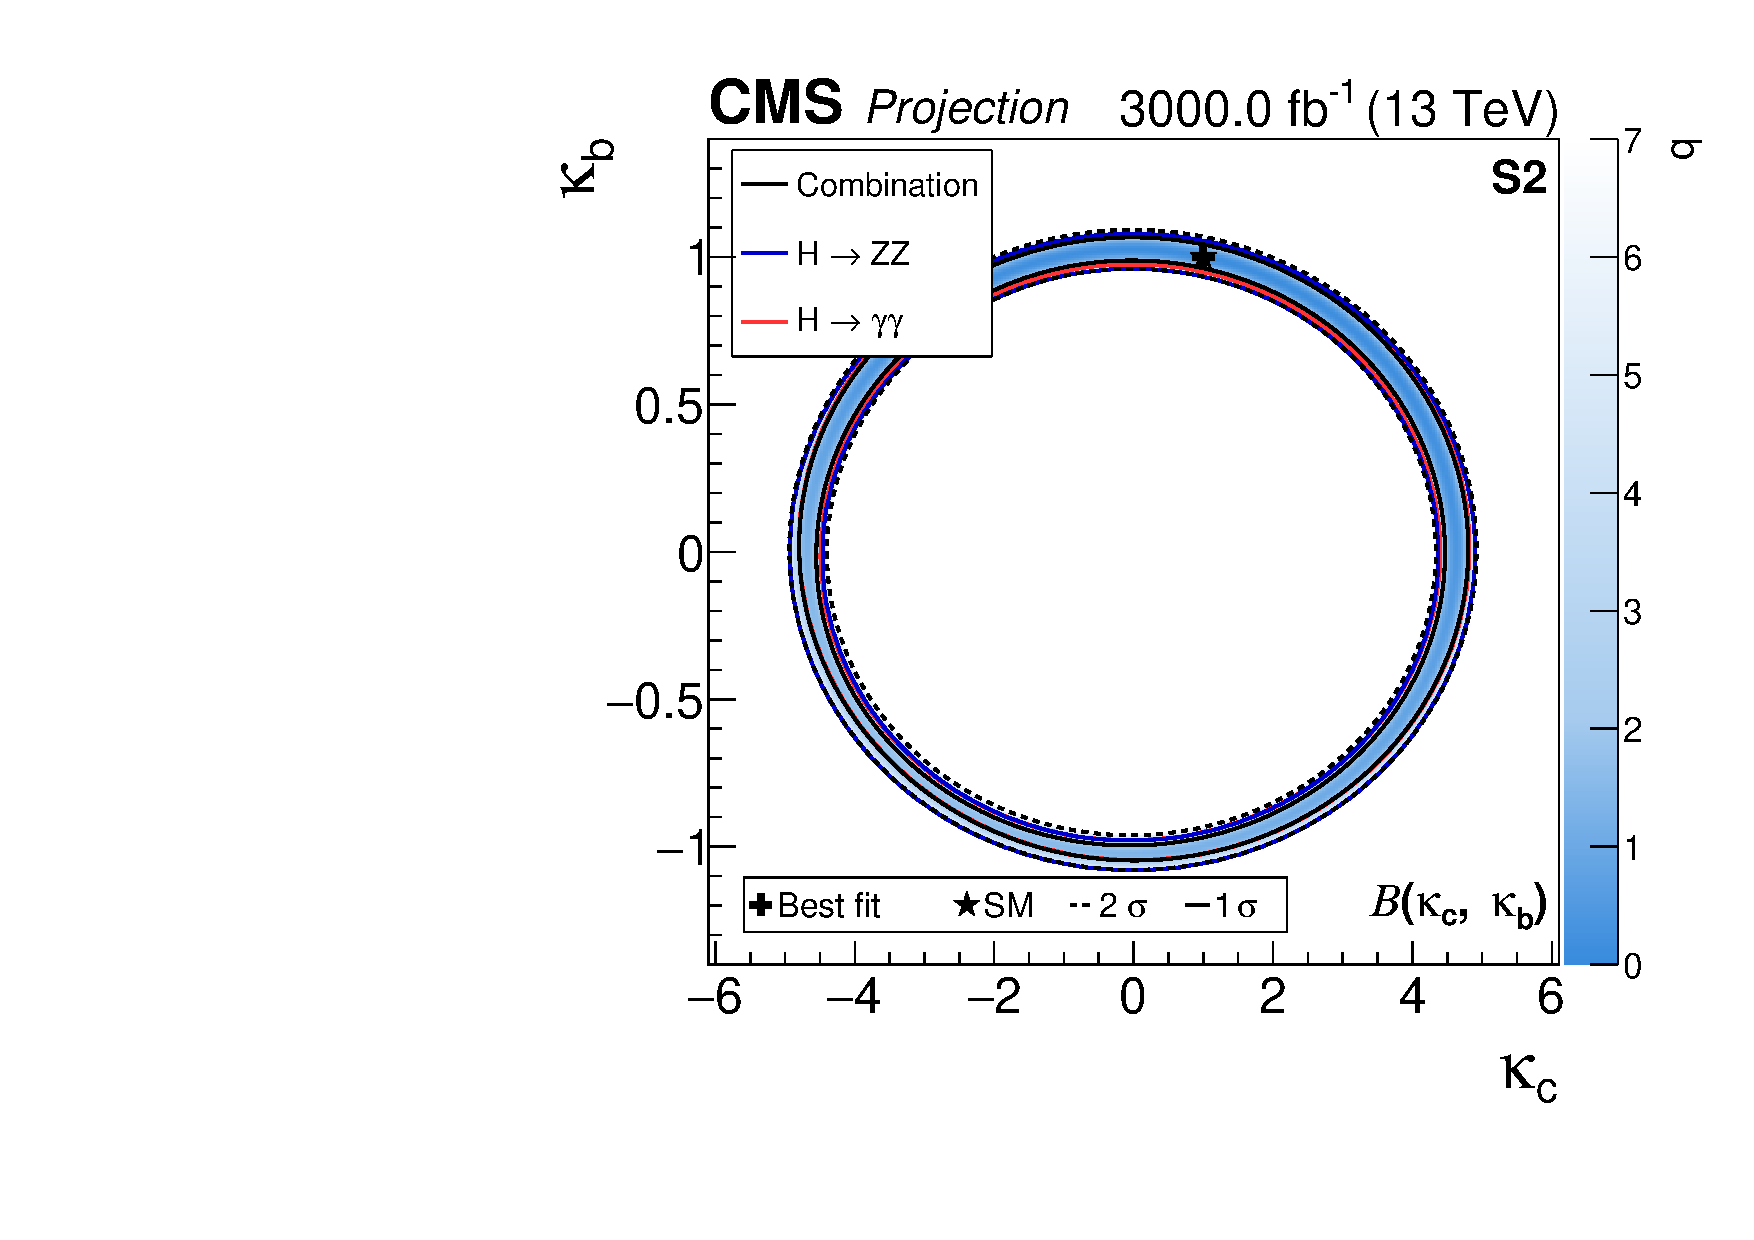
\includegraphics[width=0.49\linewidth]{\main/section7/projection_kbkc_plot_couplingdependentBRs_scenario2.pdf}
    % 
    \caption{
        Simultaneous fit to data for $\kappab$ and $\kappac$, assuming a coupling dependence of the branching fractions for Scenario 1 (\cmsLeft) and Scenario 2 (\cmsRight).
        % 
        The one standard deviation contour is drawn for the combination ($\hgg$ and $\hzz$), the $\hgg$ channel, and the $\hzz$ channel in black, red, and blue, respectively.
        % 
        For the combination the two standard deviation contour is drawn as a black dashed line, and the negative log-likelihood value on the coloured axis.
        }
    \label{fig:kbkc_couplingdependentBRs}
  \end{center}
\end{figure}

\begin{figure}[hbtp]
  \begin{center}
    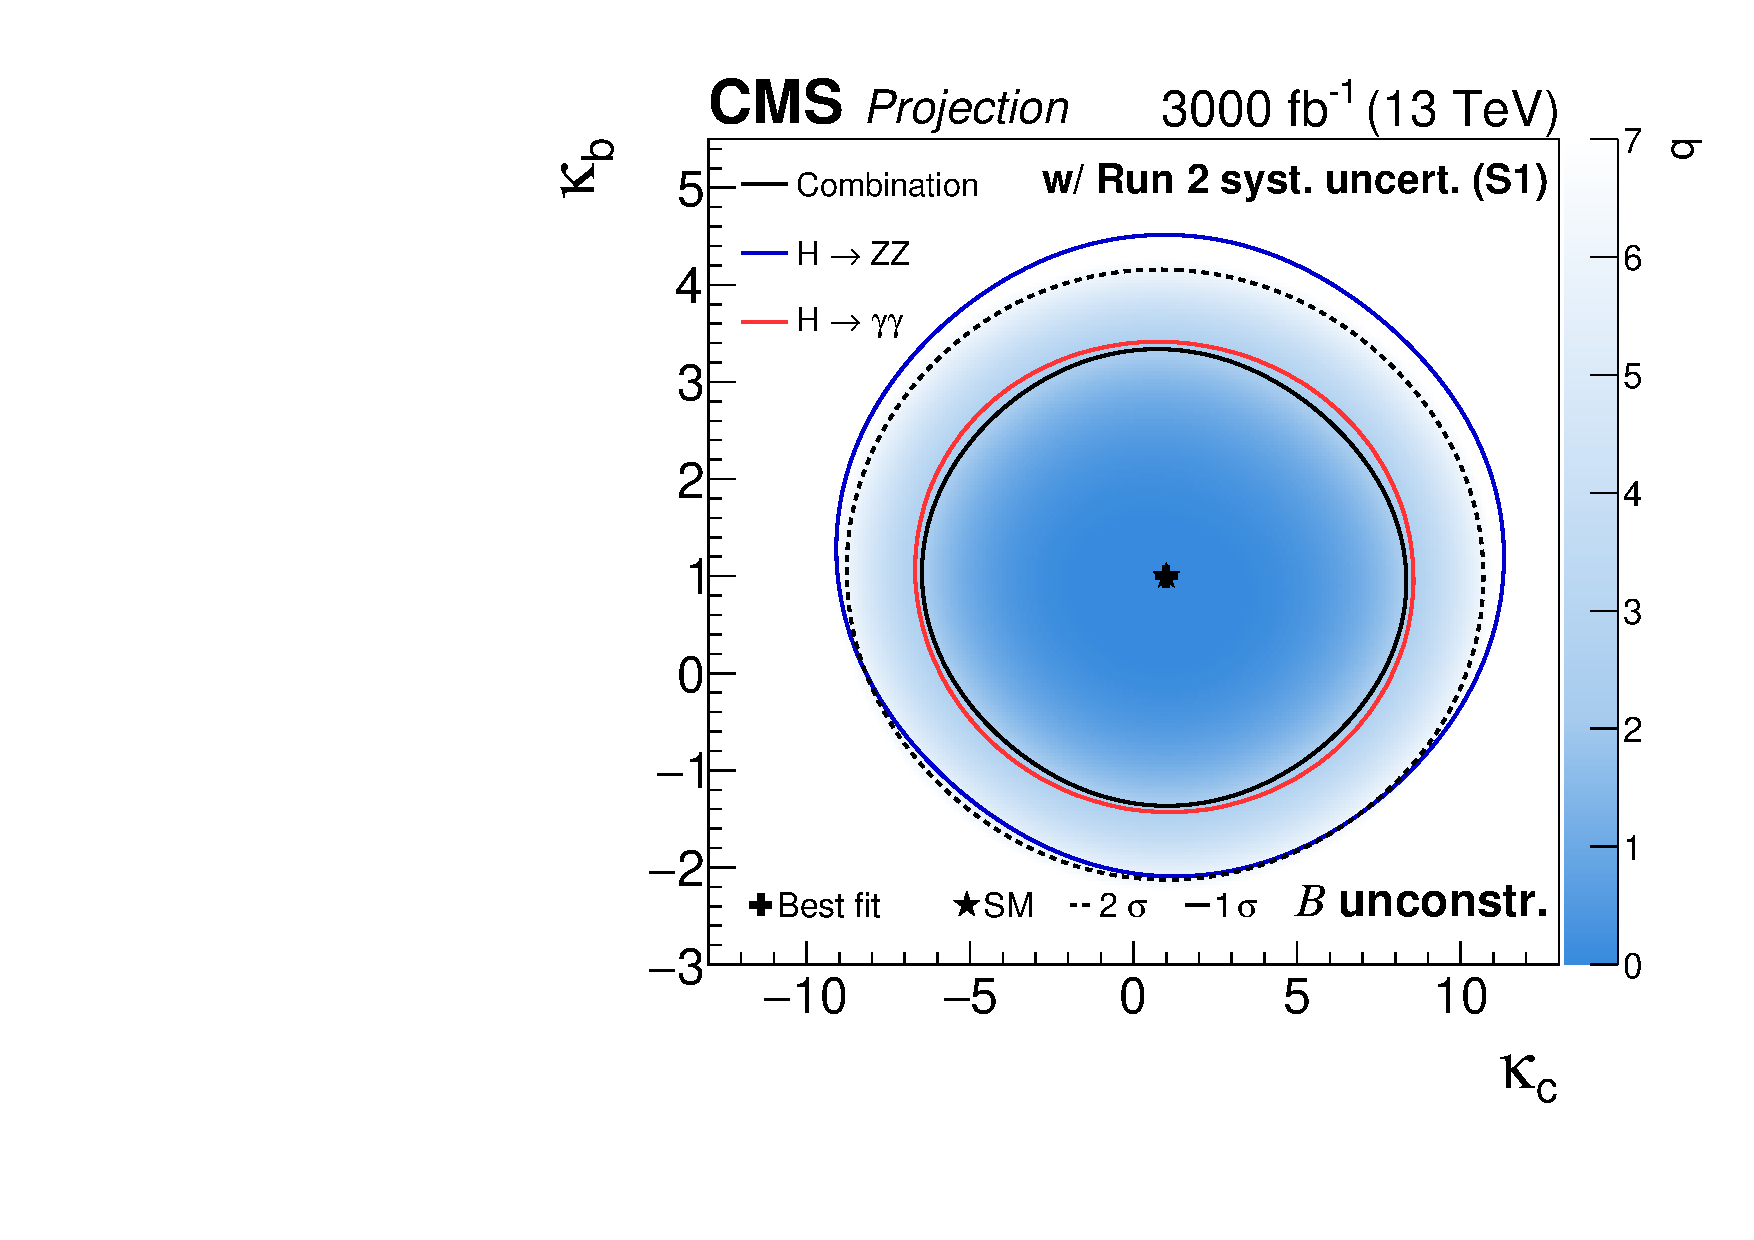
\includegraphics[width=0.49\linewidth]{\main/section7/projection_kbkc_plot_floatingBRs.pdf}
    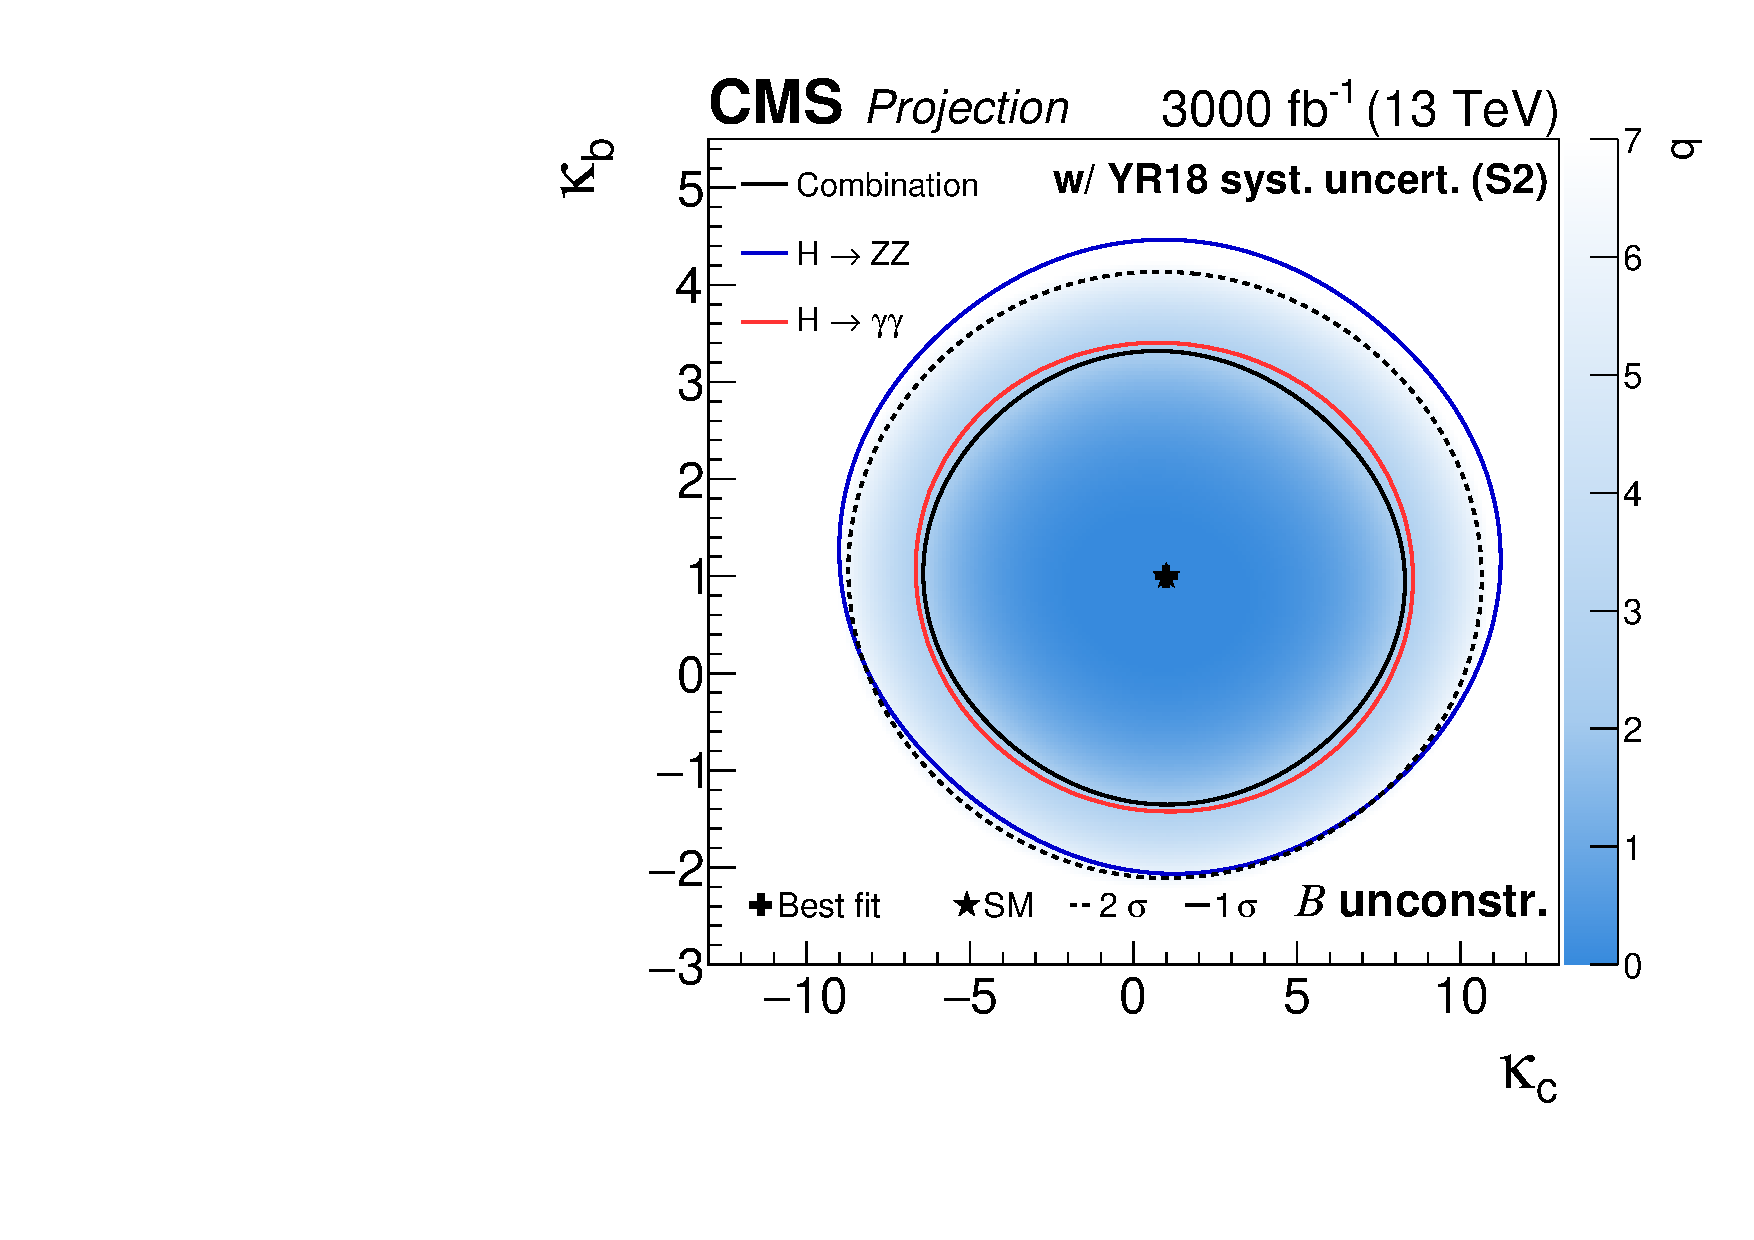
\includegraphics[width=0.49\linewidth]{\main/section7/projection_kbkc_plot_floatingBRs_scenario2.pdf}
    % 
    \caption{
        As Fig.~\ref{fig:kbkc_couplingdependentBRs}, but with the branching fractions implemented as nuisance parameters with no prior constraint.
        % 
        % Simultaneous fit to data for $\kappab$ and $\kappac$ with the branching fractions implemented as nuisance parameters with no prior constraint for Scenario 1 (\cmsLeft) and Scenario 2 (\cmsRight).
        % % 
        % The one standard deviation contour is drawn for the combination ($\hgg$ and $\hzz$), the $\hgg$ channel, and the $\hzz$ channel in black, red, and blue, respectively.
        % % 
        % For the combination the two standard deviation contour is drawn as a black dashed line, and the negative log-likelihood value on the coloured axis.
        }
    \label{fig:kbkc_floatingBRs}
  \end{center}
\end{figure}


%%%%%%%%%%%%%%%%%%%%%%%%%%%%%%%%%%%%%%%%%%%%%%%%%%%%%%%%%%%%%%%%%%%%%%%%%%%%%%%%%%%%%%%%%%%%
\subsection{$W^\pm h$ charge asymmetry}
%%%%%%%%%%%%%%%%%%%%%%%%%%%%%%%%%%%%%%%%%%%%%%%%%%%%%%%%%%%%%%%%%%%%%%%%%%%%%%%%%%%%%%%%%%%%

The $W^\pm h$ charge asymmetry, introduced in~\cite{Yu:2016rvv}, is a
new, production-based probe for constraining the light quark Yukawa
couplings.  In contrast to decay-based probes, which rely on rare or
subdominant Higgs decay modes, production-based probes can take
advantage of the dominant Higgs decays with high signal-to-background
ratios.  

The main observable is the charge asymmetry between $W^+ h$ and $W^-$
production,
%
\begin{align}
	A 
= 	\frac{ \sigma (W^+ h) - \sigma (W^- h)}
	{\sigma (W^+ h) + \sigma (W^- h) } \, ,
\end{align}
%
In the SM, the inclusive HE-LHC charge asymmetry is expected to be $17.3\%$, while the HL-LHC charge asymmetry is expected to be $21.6\%$.  In either
case, the charge asymmetry is driven by the proton PDFs and the fact
that the dominant $W^\pm h$ production mode stems from Higgs bosons
radiating from $W^\pm$ intermediate lines, where the Yukawa-mediated
diagrams are negligible.  If the quark Yukawas are not SM-like,
however, the charge asymmetry can either increase or decrease,
depending on the overall weight of the relevant PDFs.  In particular,
the charge asymmetry will increase if the down or up quark Yukawa
couplings are large, reflecting the increased asymmetry of $u \bar{d}$
vs.~$\bar{u} d$ PDFs; the charge asymmetry will decrease if the
strange or charm Yukawa couplings are large, reflecting the symmetric
nature of $c \bar{s}$ vs.~$\bar{c} s$ PDFs.  The subleading correction
from the Cabibbo angle-suppressed PDF contributions determines the
asymptotic behavior for extremely large Yukawa enhancements.

\begin{figure}[tb!]
  \begin{center}
 % \hspace*{1.5cm} 
 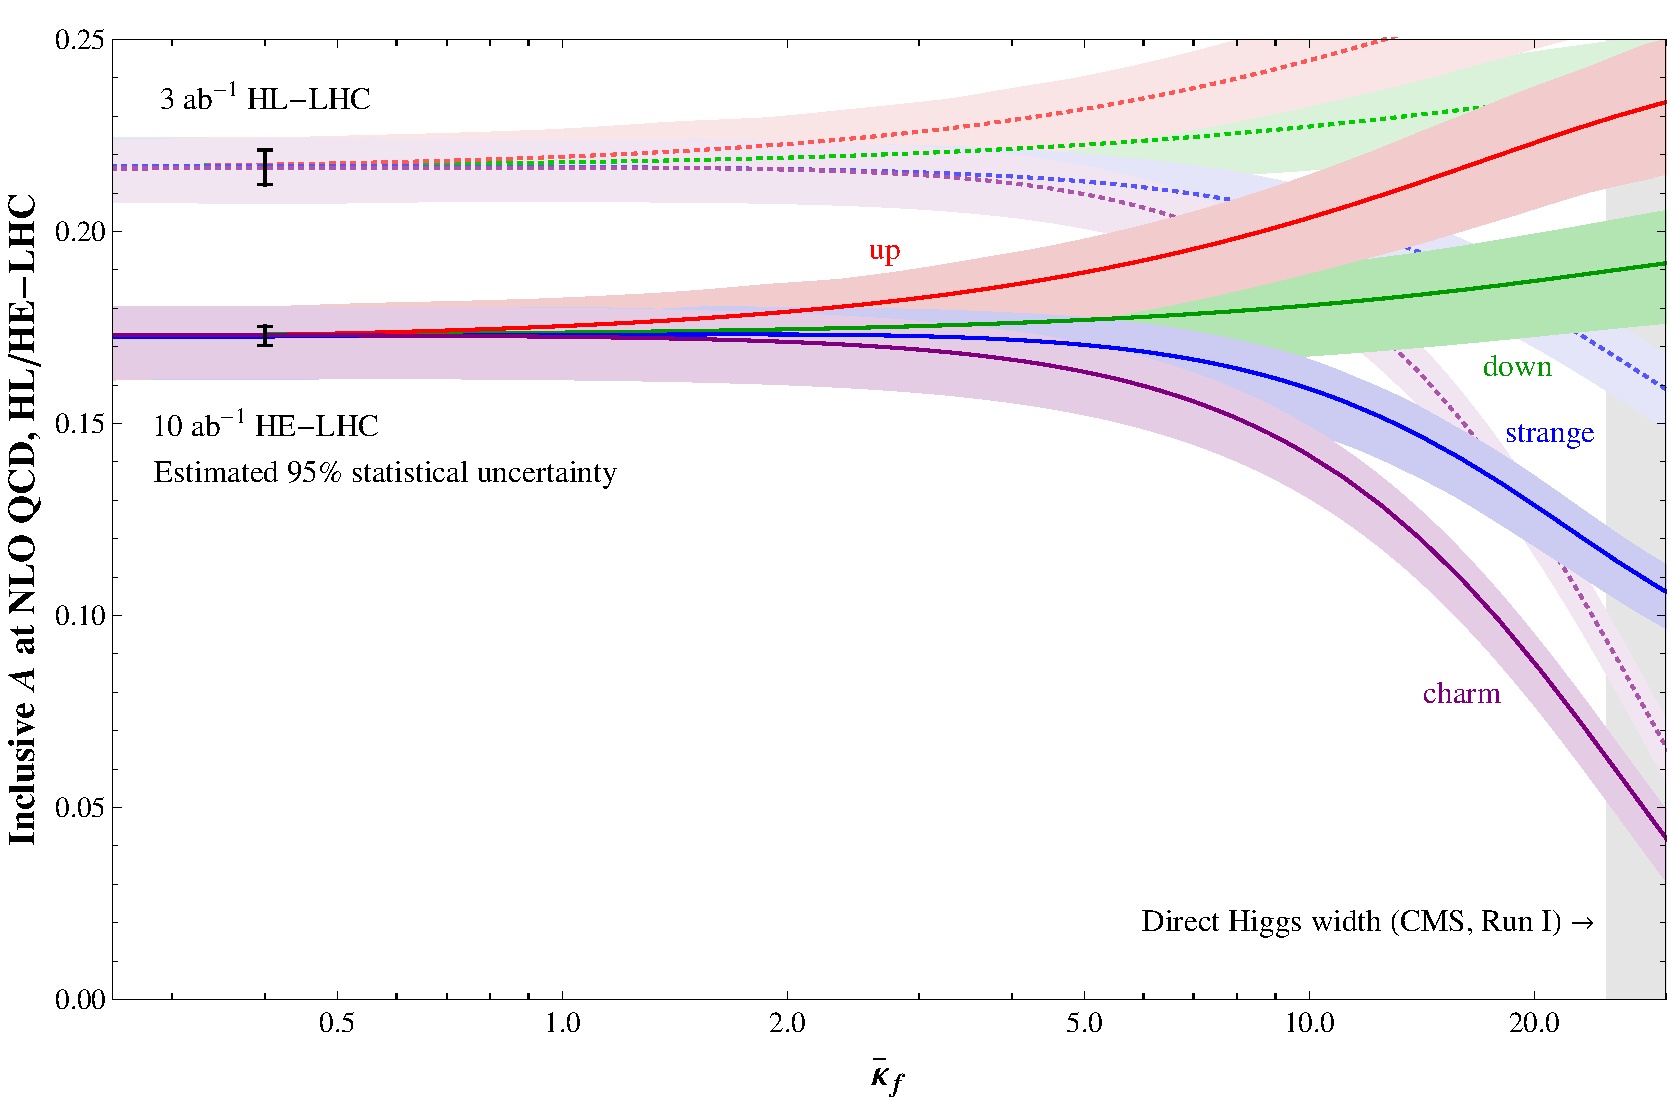
\includegraphics[width=0.6\textwidth, angle=0]{section7/AsymmetryNLO_HELHC.pdf}
 \caption{Inclusive charge asymmetry for $W^\pm h$ production at the
   27 TeV HE-LHC (solid colored bands), and 14 TeV HL-LHC (dotted
   colored bands), calculated at NLO QCD from MadGraph\_aMC@NLO using
   NNPDF 2.3 as a function of individual Yukawa rescaling factors
   $\bar{\kappa}_f$ for $f = u$ (red), $d$ (green), $s$ (blue), and
   $c$ (purple).  Shaded bands correspond to scale uncertainties at
   $1\sigma$ from individual $\sigma(W^+ h)$ and $\sigma(W^- h)$
   production, which are conservatively taken to be fully
   uncorrelated.  The expected statistical errors from this
   measurement using 10 ab$^{-1}$ of HE-LHC data and 3 ab$^{-1}$ of
   HL-LHC data are also shown.}
  \label{fig:asymmetry}
  \end{center}
\end{figure}

The effect of individual $d$, $u$, $s$, or $c$ quark Yukawa
enhancements on the inclusive charge asymmetry is shown in
Figure~\ref{fig:asymmetry}, in units of $\bar{\kappa}_f = y_f /
y_{\text{SM, b}}$, evaluated at the Higgs mass scale.  Since $W^\pm h$
production probes lower Bjorken-$x$ at the HE-LHC compared to the
HL-LHC, the expected SM charge asymmetry is lower at the higher energy
collider.  In Figure~\ref{fig:asymmetry}, we also display the expected
$0.45\%$ statistical sensitivity to the charge asymmetry coming from
an HL-LHC simulation study~\cite{Yu:2016rvv} in the $W^\pm h \to
\ell^\pm \ell^\pm jj \nu \nu$ final state.  To estimate the HE-LHC
sensitivity, we simply rescale by the appropriate luminosity ratio,
giving $0.25\%$, since we expect that the increase in both signal and
background electroweak rates to largely cancel.  We also indicate the
constraint from the direct Higgs width constraint using Run I data
from CMS~\cite{Yu:2016rvv}.  The bands denote the change in the charge
asymmetry from the varying the renormalization and factorization
scales within a factor of 2.

We see that the expected statistical sensitivity supercedes the
combined theoretical uncertainty in the PDF evaluation.  Hence, in
addition to being an important consistency check of the SM regarding
enhanced light quark Yukawa couplings, the charge asymmetry
measurement in different Higgs channels can be used to help determine
PDFs at the HE-LHC, assuming light quark Yukawa couplings are SM-like.
Separately, enhanced light quark Yukawa couplings would also generally
be expected to decrease the Higgs signal strengths, necessitating the
introduction of other new physics to be consistent with current Higgs
measurements~\cite{Yu:2016rvv}.  If the signal strengths are fixed to
SM expectation and the central prediction is used, the HE-LHC charge
asymmetry measurement could constrain $\bar{\kappa}_f \lesssim 2-3$
for up and charm quarks, and $\bar{\kappa}_f \lesssim 7$ for down or
strange quarks.

%%%% add event shap  mention: event shape, i.e. thurst,  in $e^+e^-$ collider~\cite{Gao:2016jcm}


\subsection{CP violation in Higgs couplings %(tau, ttH)
}
\noident {\it{By S. Boselli, C. M. Carloni Calame, G. Montagna, O. Nicrosini, F. Piccinini, A. Shivaji, F. Yu, Maria Moreno Llacer et al.}}

 We present prospects for studies on {\it CP}-odd couplings in the
 couplings of the Higgs boson with the eletroweak gauge bosons
 as well as in the Yukawa couplings of the Higgs boson with
 fermions, in particular with $\tau^+ \tau^-$ pairs.

\subsubsection{$VVH$ couplings}
While a large number of studies assessing the impact of {\it CP}-even
effective operators on Higgs physics is available in the literature
(see for instance the recent analysis in Ref.~\cite{Boselli:2017pef} and
references therein),
the present analysis is focused on the impact of {\it CP}-odd effective operators
on the interactions among the Higgs boson and the electroweak bosons.

In the Higgs basis, the CP-violating sector of the BSM Lagrangian affecting $VVH$ couplings is given by, {\bf YS: is there a missing tilde on the $WW$?}
%                                   
\begin{align}
\lag_{CPV} =  \frac{H}{v} \Big[
\tilde{c}_{\gamma\gamma} \frac{e^2}{4} A_{\mu\nu}\tilde{A}^{\mu\nu}
+ \tilde{c}_{Z\gamma} \frac{e\sqrt{g_1^2 + g_2^2}}{2} Z_{\mu\nu}\tilde{A}^{\mu\nu}
+ \tilde{c}_{ZZ} \frac{g_1^2 + g_2^2}{4} Z_{\mu\nu}\tilde{Z}^{\mu\nu} + \tilde{c}_{WW} \frac{g_2^2}{2} W^+_{\mu\nu}W^{-\mu\nu}\Big]
% \left. \vphantom{\half} \rq.      
\label{eqn:Hvv}
\end{align}
%
where, $g_1$ and $g_2$ are the $U(1)_Y$  and  $SU(2)_L$ gauge coupling constants. Out of the above four
parameters only three of them  are independent.
\begin{align}
 \tilde{c}_{WW} = \tilde{c}_{ZZ} + 2s_\theta^2 \tilde{c}_{Z\gamma} + s_\theta^4 \tilde{c}_{\gamma\gamma} \, .
\end{align}
The processes which are sensitive to CPV operators are the Higgstrahlung processes ($Wh$ and $Zh$), the vector boson fusion (VBF) and the Higgs decay into four\
 charged leptons ($h\to4\ell$). Here we focus on angular observables which are sensitive to CPV effects. Indeed, since the total cross-section is a CP-even quantity,  the $1/\Lambda^2$ effects of CPV operators can affect the shape of some specific kinematic distributions only.

With the present study we aim to asses the potentiality of HL/HE LHC in putting new constraints on NP arising from the bosonic CPV operators. To this end we wi\
ll show the impact of the
various processes described above in setting the upper limit on the CPV coefficients.

\begin{table*}
        \begin{center}
                \begin{tabular}{lc|ccc}
                        \multicolumn{2}{c|}{Process}     & Combination & Theory & Experimental \\ \hline \hline
                        \multirow{5}{*}{${H}\to \gamma \gamma$} &$\text{ggF}$  & 0.07 & 0.05 & 0.05 \\
                        &$\text{VBF}$ & 0.22 & 0.16 & 0.15  \\
                        &${t\overline tH}$& 0.17 & 0.12 & 0.12 \\
                        &${WH}$& 0.19 & 0.08 & 0.17 \\
                        &${ZH}$& 0.28 & 0.07 & 0.27 \\ \hline
                        \multirow{5}{*}{${H}\to {ZZ}$}                  &$\text{ggF}$& 0.06 & 0.05 & 0.04 \\
                        &$\text{VBF}$& 0.17 & 0.10 & 0.14 \\
                        &${t\overline tH}$& 0.20 & 0.12 & 0.16 \\
                        &${WH}$& 0.16 & 0.06 & 0.15 \\
                        &${ZH}$& 0.21 & 0.08 & 0.20 \\ \hline
                        \multirow{2}{*}{${H}\to {WW}$}          &$\text{ggF}$& 0.07 & 0.05 & 0.05 \\
                        &$\text{VBF}$& 0.15 & 0.12 & 0.09 \\\hline
                        ${H}\to {Z\gamma}$                                      &incl.           & 0.30 & 0.13 & 0.27           \\\hline
                        \multirow{2}{*}{${H}\to {b\bar b}$}             &${WH}$& 0.37 & 0.09 & 0.36 \\
                        &${ZH}$& 0.14 & 0.05 & 0.13 \\\hline
                        ${H}\to \tau^+ \tau^- $                                         &$\text{VBF}$ & 0.19 & 0.12 & 0.15
                \end{tabular}
                \caption{Estimated relative uncertainties on the determination of single-Higgs production channels at the high-luminosity LHC (14 TeV center of\
 mass energy and 3\,ab$^{-1}$ integrated luminosity) }\label{tab:one}
        \end{center}
\end{table*}

\subsubsection{Global fit}

We can build a $\chi^2$  as follows:
\begin{equation}
 \chi^2({\tilde c}_{Z\gamma},{\tilde c}_{ZZ}) = \sum_{i,f} \frac{(\mu_i^f -1)^2}{\sigma_{i,f}^2} \, ,
\end{equation}
The one-sigma uncertainties for the high-luminosity (14 TeV center of mass energy and 3\,ab$^{-1}$ integrated luminosity) are derived from table~\ref{tab:one}. \textit\
If we assume that the acceptance efficiency is the same at $\sqrt{s}=27$ TeV, we can also rescale the errors for the HE framework, assuming an integrated luminosity of 15\,ab$^{-1}\
$.

\subsubsection*{}{Production: Inclusive}
{\bf YS: should be some text here?}
\begin{eqnarray}
 \mu_{ZH}^{\rm 14 TeV} &=& 1 +  0.54~ {\tilde c}_{Z\gamma}^2 + 2.80~ {\tilde c}_{ZZ}^2 + 0.95~ {\tilde c}_{Z\gamma} {\tilde c}_{ZZ} \\
 \mu_{WH}^{\rm 14 TeV} &=& 1  + 0.84~ {\tilde c}_{Z\gamma}^2 + 3.87~ {\tilde c}_{ZZ}^2
   + 3.63~{\tilde c}_{Z\gamma}{\tilde c}_{ZZ} \\
 \mu_{\rm VBF}^{\rm 14 TeV} &=& 1  + 0.25~ {\tilde c}_{Z\gamma}^2 + 0.45~ {\tilde c}_{ZZ}^2
   + 0.45~{\tilde c}_{Z\gamma}{\tilde c}_{ZZ}
\end{eqnarray}

\begin{eqnarray}
 \mu_{ZH}^{\rm 27 TeV} &=& 1 +  0.63~ {\tilde c}_{Z\gamma}^2 + 3.26~ {\tilde c}_{ZZ}^2 + 1.11~ {\tilde c}_{Z\gamma} {\tilde c}_{ZZ} \\
 \mu_{WH}^{\rm 27 TeV} &=& 1 + 0.98~ {\tilde c}_{Z\gamma}^2 + 4.48~ {\tilde c}_{ZZ}^2
  + 4.16~{\tilde c}_{Z\gamma}{\tilde c}_{ZZ} \\
 \mu_{\rm VBF}^{\rm 27 TeV} &=& 1  + 0.32~ {\tilde c}_{Z\gamma}^2 + 0.67~ {\tilde c}_{ZZ}^2
  + 0.65~{\tilde c}_{Z\gamma}{\tilde c}_{ZZ}
\end{eqnarray}
The BSM predictions for VBF are derived using following cuts,
\begin{equation}
 p_T(j) > 20~{\rm GeV}, |\eta(j)| < 5, \Delta\eta_{jj} > 3, m_{jj} > 130~{\rm GeV} \nonumber
\end{equation}
The gluon fusion and $ttH$ production channels are unaffected in presence of CP-violating $VVH$
couplings.

\subsubsection*{}{Decay: Inclusive}

\begin{eqnarray}
 R_{\Gamma}(H \to 2e2\mu) &=& 1  + 0.308~ {\tilde c}_{Z\gamma}^2 + .00315~ {\tilde c}_{ZZ}^2
   + (-.00577)~{\tilde c}_{Z\gamma}{\tilde c}_{ZZ} \\
 R_{\Gamma}(H \to 4e)
 &=& R_{\Gamma}(H \to 4\mu) \nonumber \\
 &=& 1  + 3.38~ {\tilde c}_{Z\gamma}^2 + 0.00239~ {\tilde c}_{ZZ}^2
   + (-.00507)~{\tilde c}_{Z\gamma}{\tilde c}_{ZZ}
\end{eqnarray}
{\bf YS: what is $R_\Gamma$?}
The BSM coefficients in $R_{\Gamma}(H \to 4e)$ are different from those given in the Appendix~A of
Ref.~\cite{Boselli:2017pef} due to a difference in selection cuts. The above expression for Higgs decay
into $4e$ is obtained after applying a selection cut of 15\,GeV on the leading and subleading lepton pairs
of opposite sign.

In the present analysis, we assume that total Higgs decay width remains unchanged in presence of BSM. In this
case the signal strength for decay is just the ratio of decay widths in BSM and in SM.
%
\begin{eqnarray}
 \mu^{4\ell} &=& 1  + 2.06~ {\tilde c}_{Z\gamma}^2 +
 0.00272~ {\tilde c}_{ZZ}^2  -
 0.00537~ {\tilde c}_{Z\gamma} {\tilde c}_{ZZ}
\end{eqnarray}
%
\subsubsection*{}{Decay: Differential}
The kinematic variable considered in the present analysis is,
\begin{equation}
        \cos \phi =
        \frac{\left( k_{12} \times k_1\right) \cdot \left( k_{12} \times k_3 \right)}
        {\left| k_{12} \times k1 \right| \left| k_{12} × k_3 \right|}
\end{equation}


To begin with, we divide the distribution in two bins--[0:180] and [180:360]. The signal strengths for the decay in these two bins
are given by,
%
\begin{eqnarray}
 \mu^{4\ell,\phi(1)} &=& 1 +  (-0.132)~{\tilde c}_{Z\gamma} +
  (0.00265)~{\tilde c}_{ZZ}  +  (2.08)~{\tilde c}_{Z\gamma}^2  + \nonumber \\ &&
  (0.00267)~{\tilde c}_{ZZ}^2 +
  (-0.00592)~{\tilde c}_{Z\gamma} {\tilde c}_{ZZ}
\end{eqnarray}
%
\begin{eqnarray}
 \mu^{4\ell,\phi(2)} &=& 1 + (0.145)~ {\tilde c}_{Z\gamma} +
  (-0.00291)~{\tilde c}_{ZZ}  +  (2.04)~{\tilde c}_{Z\gamma}^2 + \nonumber \\ &&
  (0.00276)~{\tilde c}_{ZZ}^2 +
  (-0.00607)~{\tilde c}_{Z\gamma} {\tilde c}_{ZZ}
\end{eqnarray}
%
{\it We will consider more than two bins to gain a better sensitivity on the linear coefficients.}

\begin{figure}
\centering
 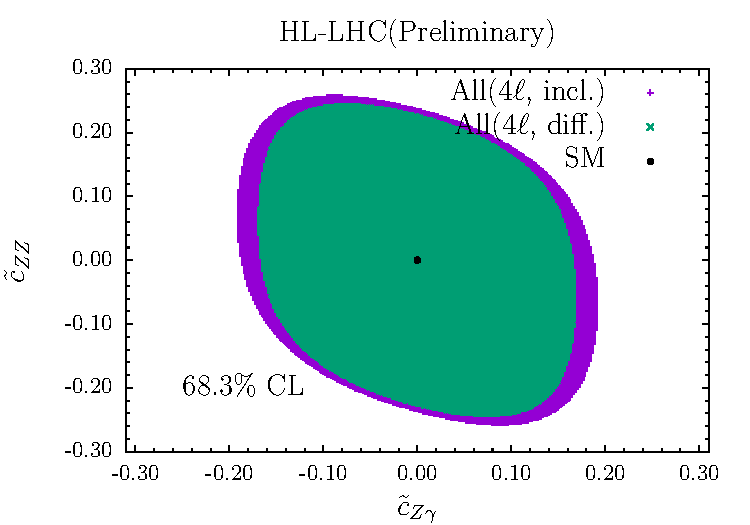
\includegraphics[scale=0.5]{tCza-tCzz-4l-all-HL}
 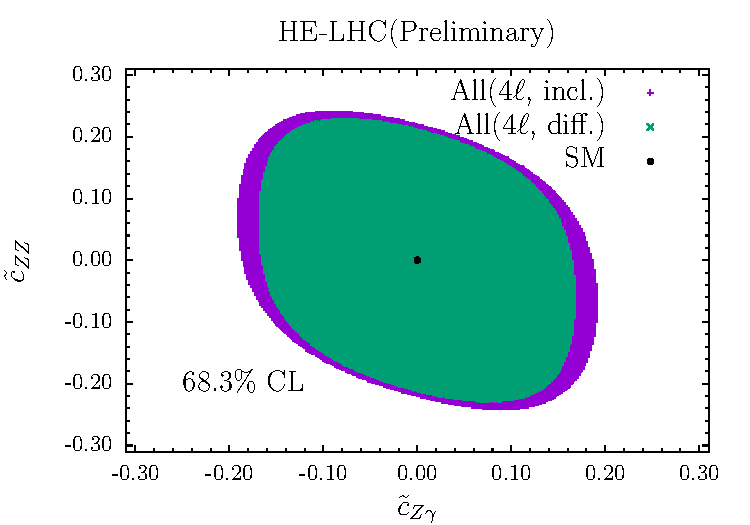
\includegraphics[scale=0.5]{tCza-tCzz-4l-all-HE}
 \caption{A comparison of global fits using inclusive (purple) and differential (green) information in the
 definition of signal strength for the $H \to 4\ell$. The fit is obtained using all the production channels.
 In both cases, the uncertainties are kept same. The right plot thus shows the shear effect
 of increasing the centre-of-mass energy.}
\end{figure}



\subsubsection{$h \to \tau^+ \tau^-$}

The most promising direct probe of CP violation in fermionic Higgs
decays is the $\tau^+ \tau^-$ decay channel, which benefits from a
relatively large $\tau$ Yukawa giving a SM branching fraction of
$6.3\%$. Measuring the CP violating phase in the tau Yukawa requires a measurement of the linear polarizations of both $\tau$ leptons and and the azimuthal angle between them. This can be done by analyzing tau substructure, namely the angular distribution of the various components of the tau decay products.

The main $\tau$ decay modes studied include $\tau^\pm \to
\rho^\pm (770) \nu$, $\rho^\pm \to \pi^\pm \pi^0$~\cite{Bower:2002zx,
  Desch:2003mw, Desch:2003rw, Harnik:2013aja, Askew:2015mda,
  Jozefowicz:2016kvz} and $\tau^\pm \to \pi^\pm
\nu$~\cite{Berge:2008wi, Berge:2008dr, Berge:2011ij}.  Assuming CPT
symmetry, collider observables for CP violation must be built from
differential distributions based on triple products of three-vectors.
In the first case, $h \to \pi^\pm \pi^0 \pi^\mp \pi^0 \nu \nu$,
angular distributions built only from the outgoing charged and neutral
pions are used to determine the CP properties of the initial $\tau$
Yukawa coupling.  In the second case, $h \to \pi^\pm \pi^\mp \nu \nu$,
there are not enough reconstructible independent momenta to construct an observable sensitive to CP violation, requiring additional kinematic information such as the $\tau$ decay impact parameter.

In the kinematic limit when each outgoing neutrino is taken to be
collinear with its corresponding reconstructed $\rho^\pm$ meson, the
acoplanarity angle, denoted $\Phi$, between the two decay planes
spanned by the $\rho^\pm \to \pi^\pm \pi^0$ decay products is exactly
analogous to the familiar acoplanarity angle from $h \to 4 \ell$
CP-property studies.  Hence, by measuring the $\tau$ decay products in
the single-prong final state, suppressing the irreudicible $Z \to
\tau^+ \tau^-$ and reducible QCD backgrounds, and reconstructing the
acoplanarity angle of $\rho^+$ vs.~$\rho^-$, the differential
distribution in $\Phi$ gives a sinusoidal shape whose maxima and
minima correspond to the CP-phase in the $\tau$ Yukawa coupling.  

An optimal observable using the colinear approximation was derived in~\cite{Harnik:2013aja}. Assuming 70\% efficiency for tagging hadronic $\tau$ final states, and
neglecting detector effects, the estimated sensitivity for the
CP-violating phase of the $\tau$ Yukawa coupling using 3 ab$^{-1}$ at
the HL-LHC is 8.0$^\circ$.  A more sophisticated
analysis~\cite{Askew:2015mda} found that detector resolution effects
on the missing transverse energy distribution degrade the expected
sensitivity considerably, and as such, about 1 ab$^{-1}$ is required
to distinguish a pure scalar coupling (CP phase is zero) from a pure
pseudoscalar coupling (CP phase is $\pi/2$).

At the HE-LHC, the increased signal cross section for Higgs production
is counterbalanced by the increased background rates, and so the main
expectation is that improvements in sensitivity will be driven by the
increased luminosity and more optimized experimental methodology.
Rescaling with the appropriate luminosity factors, the optimistic
sensitivity to the $\tau$ Yukawa phase from acoplanarity studies is
4-5$^\circ$, while the more conservative estimate is roughly an order
of magnitude worse.

\subsubsection{$ t\,\bar{t}\,h$}

CP violation in the top quark-Higgs coupling is strongly constrained by EDM measurements and Higgs rate measurements~\cite{Brod:2013cka}. However, these constraints assume that the light quark Yukawa couplings and $hWW$ couplings have their SM values. If this is not the case, the constraints the phase of the top Yukawa coupling relax.
    
Assuming the EDM and Higgs rate  constraints can be avoided, the CP structure of the top quark Yukawa can be probed directly in $pp \to t\bar t h$. Many simple observables, such as $m_{t\bar t h}$ and $p_{T,h}$ are sensitive to the CP structure, but require reconstructing the top quarks and Higgs.

Some $t\bar t h$ observables have been proposed recently that access the CP structure without requiring full event reconstruction. These in include the azimuthal angle between the two leptons in a fully leptonic $t/bar{t}$ decay with the additional requirement that the $p_{T,h} > 200\, \text{GeV}$~\cite{Buckley:2015vsa}, and the angle between the leptons (again in a fully leptonic $t/\bar t$ system) projected onto the plane perpendicular to the $h$ momentum~\cite{Boudjema:2015nda}. These observables only require that the Higgs is reconstructed and are inspired by the sensitivity of $\Delta \phi_{\ell^+\ell^-}$ to top/anti-top spin correlations in $pp \to t\bar t$~\cite{Mahlon:1995zn}. The sensitivity of both of these observables improves at higher Higgs boost (and therefore higher energy), making them promising targets for the HE-LHC, though no dedicated studies have been carried out to date.

\subsection{Summary}

{\bf YS: add summary }

\end{document}
